%Version 3.1 December 2024
% See section 11 of the User Manual for version history
%
%%%%%%%%%%%%%%%%%%%%%%%%%%%%%%%%%%%%%%%%%%%%%%%%%%%%%%%%%%%%%%%%%%%%%%
%%                                                                 %%
%% Please do not use \input{...} to include other tex files.       %%
%% Submit your LaTeX manuscript as one .tex document.              %%
%%                                                                 %%
%% All additional figures and files should be attached             %%
%% separately and not embedded in the \TeX\ document itself.       %%
%%                                                                 %%
%%%%%%%%%%%%%%%%%%%%%%%%%%%%%%%%%%%%%%%%%%%%%%%%%%%%%%%%%%%%%%%%%%%%%

%%\documentclass[referee,sn basic]{sn-jnl}% referee option is meant for double line spacing

%%=======================================================%%
%% to print line numbers in the margin use lineno option %%
%%=======================================================%%

%%\documentclass[lineno,pdflatex,sn basic]{sn jnl}% Basic Springer Nature Reference Style/Chemistry Reference Style

%%=========================================================================================%%
%% the documentclass is set to pdflatex as default. You can delete it if not appropriate.  %%
%%=========================================================================================%%

%%\documentclass[sn basic]{sn jnl}% Basic Springer Nature Reference Style/Chemistry Reference Style

%%Note: the following reference styles support Namedate and Numbered referencing. By default the style follows the most common style. To switch between the options you can add or remove �Numbered� in the optional parenthesis. 
%%The option is available for: sn basic.bst, sn chicago.bst%  
 
%%\documentclass[pdflatex,sn nature]{sn jnl}% Style for submissions to Nature Portfolio journals
%%\documentclass[pdflatex,sn basic]{sn jnl}% Basic Springer Nature Reference Style/Chemistry Reference Style
\documentclass[pdflatex,sn-mathphys-num]{sn-jnl}% Math and Physical Sciences Numbered Reference Style
%%\documentclass[pdflatex,sn mathphys ay]{sn jnl}% Math and Physical Sciences Author Year Reference Style
%%\documentclass[pdflatex,sn aps]{sn jnl}% American Physical Society (APS) Reference Style
%%\documentclass[pdflatex,sn vancouver num]{sn jnl}% Vancouver Numbered Reference Style
%%\documentclass[pdflatex,sn vancouver ay]{sn jnl}% Vancouver Author Year Reference Style
%%\documentclass[pdflatex,sn apa]{sn jnl}% APA Reference Style
%%\documentclass[pdflatex,sn chicago]{sn jnl}% Chicago based Humanities Reference Style
%%%% Standard Packages
%%<additional latex packages if required can be included here>
\usepackage{tabularx} % in preamble
\usepackage{booktabs} % optional, but cleaner
\usepackage{graphicx}%
\usepackage{multirow}%
\usepackage{amsmath,amssymb,amsfonts}%
\usepackage{amsthm}%
\usepackage{mathrsfs}%
\usepackage[title]{appendix}%
\usepackage{xcolor}%
\usepackage{textcomp}%
\usepackage{manyfoot}%
\usepackage{booktabs}%
\usepackage{algorithm}%
\usepackage{algorithmicx}%
\usepackage{algpseudocode}%
\usepackage{listings}%
\usepackage{placeins}
%%%%

%%%%%=============================================================================%%%%
%%%%  Remarks: This template is provided to aid authors with the preparation
%%%%  of original research articles intended for submission to journals published 
%%%%  by Springer Nature. The guidance has been prepared in partnership with 
%%%%  production teams to conform to Springer Nature technical requirements. 
%%%%  Editorial and presentation requirements differ among journal portfolios and 
%%%%  research disciplines. You may find sections in this template are irrelevant 
%%%%  to your work and are empowered to omit any such section if allowed by the 
%%%%  journal you intend to submit to. The submission guidelines and policies 
%%%%  of the journal take precedence. A detailed User Manual is available in the 
%%%%  template package for technical guidance.
%%%%%=============================================================================%%%%

%% as per the requirement new theorem styles can be included as shown below
\theoremstyle{thmstyleone}%
\newtheorem{theorem}{Theorem}%  meant for continuous numbers
%%\newtheorem{theorem}{Theorem}[section]% meant for sectionwise numbers
%% optional argument [theorem] produces theorem numbering sequence instead of independent numbers for Proposition
\newtheorem{proposition}[theorem]{Proposition}% 
%%\newtheorem{proposition}{Proposition}% to get separate numbers for theorem and proposition etc.

\theoremstyle{thmstyletwo}%
\newtheorem{example}{Example}%
\newtheorem{remark}{Remark}%

\theoremstyle{thmstylethree}%
\newtheorem{definition}{Definition}%

\raggedbottom
%%\unnumbered% uncomment this for unnumbered level heads

\begin{document}

\title[GPU Acceleration in Computational Lithography: Taxonomy, Survey, and
Roadmap
]{GPU Acceleration in Computational Lithography: Taxonomy, Survey, and
Roadmap
}

%%=============================================================%%
%% GivenName	 > \fnm{Joergen W.}
%% Particle	 > \spfx{van der}  > surname prefix
%% FamilyName	 > \sur{Ploeg}
%% Suffix	 > \sfx{IV}
%% \author*[1,2]{\fnm{Joergen W.} \spfx{van der} \sur{Ploeg} 
%%  \sfx{IV}}\email{iauthor@gmail.com}
%%=============================================================%%

\author*[1]{\fnm{Shadi} \sur{Alawneh}}\email{shadialawneh@oakland.edu}

\author[1]{\fnm{Mayuresh} \sur{Karandikar}}\email{mvkarandikar@oakland.edu}
\equalcont{These authors contributed equally to this work.}


\affil[1]{\orgdiv{Electrical and Computer Engineering Department}, \orgname{Oakland University}, \orgaddress{ \city{Rochester Hills}, \state{Michigan}, \country{USA}}}

%\affil[2]{\orgdiv{Electrical and Computer Engineering Department}, \orgname{Oakland University}, \orgaddress{ \city{Rochester Hills}, \state{Michigan}, \country{USA}}}

%%==================================%%
%% Sample for unstructured abstract %%
%%==================================%%

\abstract
{

\textcolor{blue}{In modern semiconductor manufacuring, computational lithogrpaphy plays more and more important role and has become a key enabler in keeping up with growing demands of the field. However, as wafer sizes shrink, and feature density increses, traditional forms of computational lithography has started facing limitations.} Recent advancements in General-Purpose GPU (GPGPU) computing have transformed this landscape, enabling the transition from traditional CPU-based heuristics to massive, physics-based optimization. This paper provides a comprehensive survey of the GPU-accelerated computational lithography ecosystem. We first establish a multi-dimensional taxonomy covering application domains such as Inverse Lithography Technology (ILT) and EUV modeling alongside their underlying numerical algorithms. We then detail the GPU-resident computational workflow, illustrating how iterative optimization loops minimize host-device bottlenecks. Finally, we analyze specific GPU acceleration strategies, from SIMT parallelism and memory-aware tiling to emerging AI-physics hybrids. By synthesizing these elements, this review offers a roadmap for researchers to navigate the current state-of-the-art and identifies future trajectories in GPU-driven lithographic optimization.



% Computational lithography is a critical enabler of advanced semiconductor manufacturing, supporting mask correction, optical imaging, and resist process modeling at nanoscale technology nodes. As feature sizes shrink, workloads associated with optical proximity correction (OPC), inverse lithography technology (ILT), source–mask optimization (SMO), and stochastic resist simulation scale superlinearly, overwhelming traditional CPU-centric workflows. Recent advances in graphics processing units (GPUs) and heterogeneous cluster architectures have fundamentally transformed this landscape by offering massive parallelism, high memory bandwidth, and improved energy efficiency for lithography workloads dominated by FFT-based imaging, partial differential equation solvers, and iterative inverse optimization.

% This survey presents a comprehensive taxonomy of GPU-accelerated computational lithography from a high-performance computing perspective. We categorize prior work across application domains, numerical methods, and system designs, including multi-GPU nodes and GPU clusters. Drawing on academic research and industrial platforms such as NVIDIA cuLitho, we analyze scalability trends, memory and communication bottlenecks, precision considerations, and reproducibility challenges. We further outline open challenges and a roadmap for scalable, energy-efficient lithography on modern GPU-accelerated clusters.    

\begin{figure}[t]
  \centering
  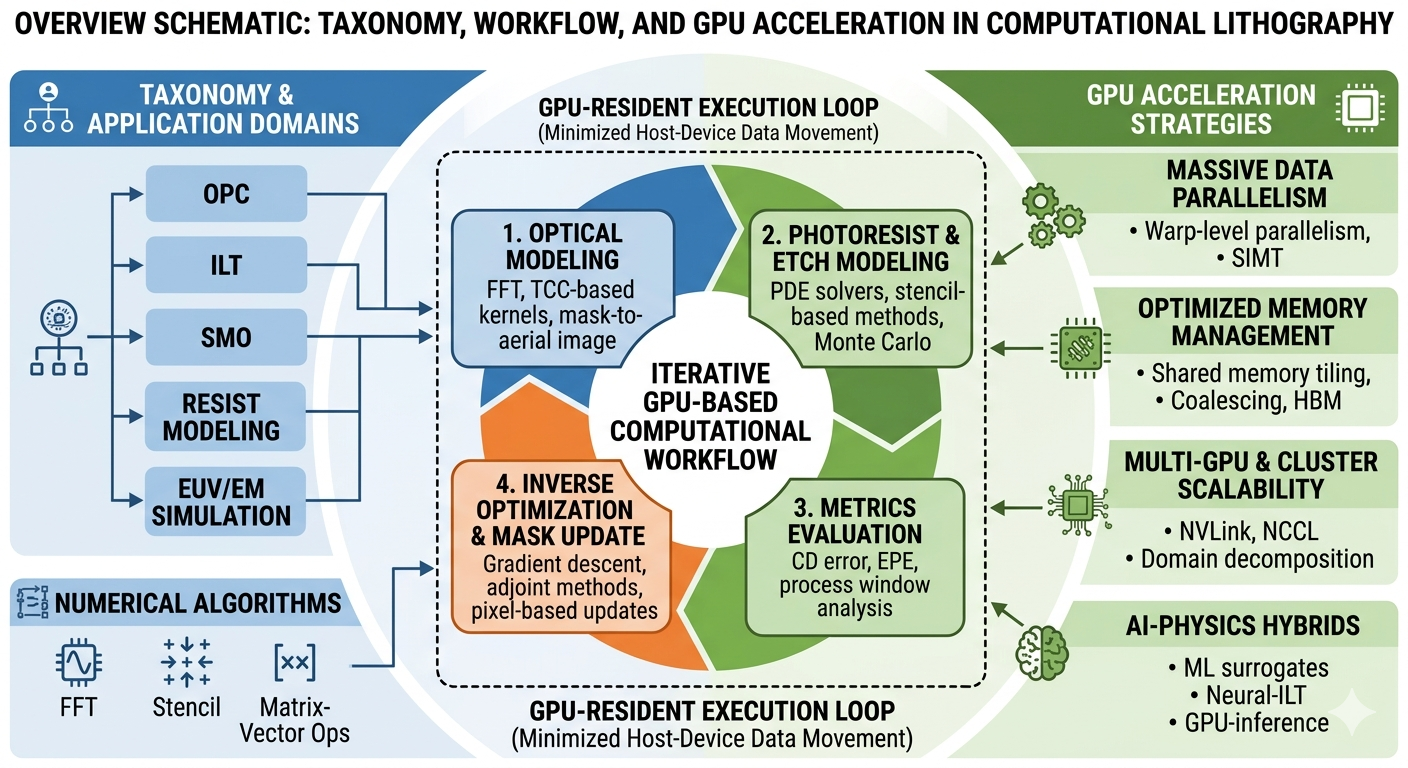
\includegraphics[width=1.0\linewidth]{images/summary.png}
  \caption{Pillars of GPU enabled Computational lithography}
  \label{fig:Comptuational Lithography Pillars}
\end{figure}

}

\keywords{GPU Computing, Computational Lithography, Heterogeneous Clusters, Inverse Lithography Technology (ILT), High-Performance Computing (HPC), Semiconductor Manufacturing}


\maketitle

\section{Introduction}\label{sec1}
Computational lithography has become a cornerstone of modern semiconductor manufacturing, enabling accurate pattern transfer from photomasks to silicon wafers as feature sizes approach fundamental physical limits. Techniques such as optical proximity correction (OPC), inverse lithography technology (ILT), and source–mask optimization (SMO) are now indispensable components of modern lithographic workflows \cite{capodieci2006optical,cecil2022advances,chen2022label}. However, these techniques rely on repeated, high-dimensional numerical simulations whose computational cost scales superlinearly with layout complexity, mask resolution, and process window exploration, making computational lithography a major scalability bottleneck.

The computational burden of modern lithography arises from several tightly coupled components. Forward imaging relies heavily on FFT-based convolution and electromagnetic field calculations to model diffraction and partial coherence effects \cite{Zheng2023,1953RSPSA}. Resist modeling further increases computational cost through reaction–diffusion partial differential equation solvers and stochastic Monte Carlo simulations, particularly in extreme ultraviolet (EUV) lithography where photon shot noise becomes significant \cite{Gallatin2005,2017JMM&M}. Inverse optimization techniques such as ILT and SMO amplify this burden by requiring thousands of iterations of forward simulation under varying constraints and objectives \cite{cecil2022advances,Ma19}. At full-chip scale, these workflows can translate into hundreds of CPU-years of computation, rendering traditional CPU-centric approaches increasingly impractical for production environments.

Graphics processing units (GPUs) have emerged as a transformative computing platform for addressing these challenges. Rather than serving as incremental accelerators, GPUs act as structural enablers for computational lithography by naturally matching the massive data parallelism inherent in pixel-level imaging, stencil-based resist solvers, and iterative inverse optimization loops \cite{4490127,kirk10}. Over the past two decades, academic research has demonstrated substantial GPU acceleration for FFT-based optical simulation and OPC/ILT workflows \cite{ZHANG2015176,Zheng2024,yang2024gpuacceleratedinverselithographyhigh}. These developments have culminated in recent industrial adoption, most notably NVIDIA’s cuLitho platform, which reports up to 40× runtime speedups and order-of-magnitude improvements in energy efficiency compared to CPU-based lithography flows \cite{Singh}. Figure~\ref{fig:gpu_pipeline} illustrates a representative GPU-centric computational lithography pipeline, highlighting the tight coupling between forward simulation, resist modeling, and inverse optimization within a fully device-resident execution model.

\begin{figure}[t]
  \centering
  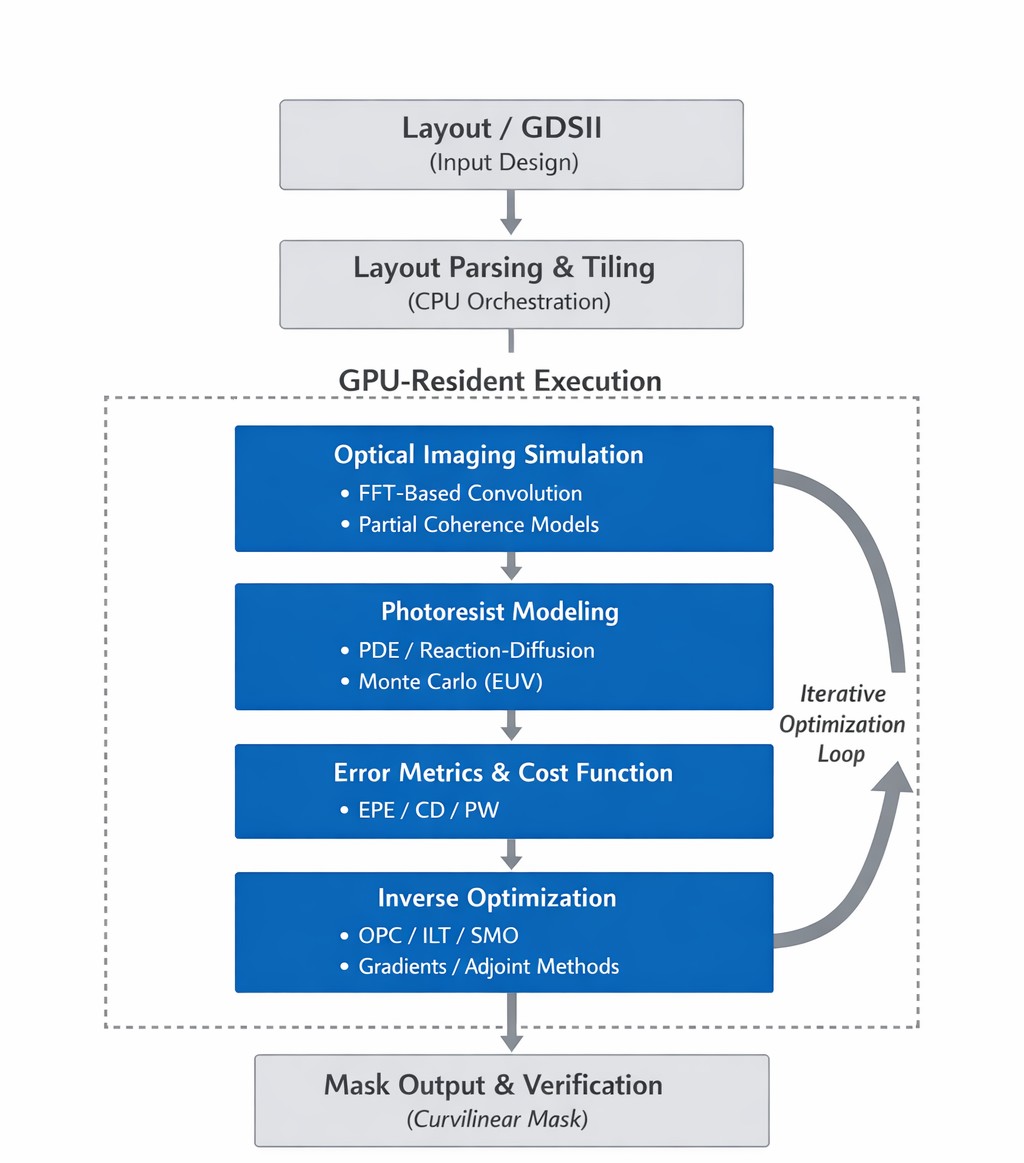
\includegraphics[width=0.7\linewidth]{images/fig1.png}
  \caption{Conceptual GPU-centric computational lithography pipeline. Optical imaging, photoresist modeling, error evaluation, and inverse optimization are executed as a fully GPU-resident iterative workflow, minimizing data movement and enabling efficient single-GPU, multi-GPU, and cluster-scale execution.}
  \label{fig:gpu_pipeline}
\end{figure}



Beyond performance, energy efficiency has become another dominant constraint shaping computational lithography system design. Modern high-performance computing systems operate under strict power budgets, particularly as they approach exascale capabilities. Lithography workloads, which require repeated simulation across large design spaces and process conditions, magnify the cost of inefficient execution. GPU-accelerated clusters provide significantly higher arithmetic throughput and memory bandwidth per watt than CPU-only systems, making them well suited for sustained, large-scale lithographic computation \cite{kirk10,10.5555/1964238.1964240}.

Equally important is how GPU acceleration is integrated into the overall lithography workflow. Early approaches often offloaded isolated kernels, such as FFTs, while retaining control logic and intermediate data on the CPU \cite{ZHANG2015176}. Such designs suffer from significant overhead due to repeated host–device data transfers. More recent frameworks emphasize full-pipeline GPU residency, where optical simulation, resist modeling, and inverse optimization remain device-resident across iterations. \textcolor{blue}{ These methods compensate for CPU-GPU transfer latency by parallelizing compute and transfer stages and pipelining them. Apart from reducing communication overhead, this also improves energy efficiency, and enables more effective multi-GPU scaling on cluster architectures }\cite{Nickolls08}.

Motivated by these developments, this paper presents a comprehensive survey of GPU-accelerated computational lithography. We provide a taxonomy spanning application domains, numerical methods, and system architectures; synthesize trends across academic research and industrial deployment; and analyze key challenges related to scalability, memory behavior, numerical precision, and reproducibility. Finally, we outline a roadmap for future research at the intersection of GPU-accelerated clusters, high-performance computing, and next-generation semiconductor manufacturing. Unlike prior surveys that focus primarily on lithography physics or OPC algorithms, this work frames computational lithography explicitly as a high-performance and cluster computing problem.

\section{Foundations of Computational Lithography}
\subsection{Optical Imaging and Diffraction}
Optical imaging in computational lithography is most commonly modeled using a Fourier optics framework, in which the lithographic system is represented as a sequence of linear transformations from the mask plane to the pupil plane and ultimately to the wafer plane. In this formulation, the mask pattern is treated as a spatially varying complex field whose diffraction spectrum is filtered by the projection optics before being reconstructed as an aerial image on the wafer. This approach is grounded in the partially coherent imaging theory introduced by Hopkins and later refined for practical lithography simulation using frequency-domain formulations \cite{Hopkins88,Mack2007FundamentalPO}. The Fourier optics perspective naturally decomposes the physical modeling problem into a small number of mathematically well-defined operations—primarily Fourier transforms, spectral filtering, and inverse transforms—which form the computational core of lithography simulation.

At the heart of this workflow is the use of FFT-based convolution to compute aerial images efficiently. For partially coherent illumination, which is standard in modern lithography systems, the aerial image is formed by aggregating contributions from multiple source points or illumination modes, each requiring a Fourier-domain propagation through the optical system \cite{Mack2007FundamentalPO,Wong2001ResolutionET}. While partial coherence improves modeling fidelity, it significantly increases computational cost by requiring repeated FFT-based evaluations across source distributions, focus conditions, and aberration settings. Consequently, optical simulation often dominates runtime in OPC, ILT, and SMO workflows \cite{Wong2001ResolutionET,capodieci2006optical}.

From a computational standpoint, these operations exhibit a high degree of data parallelism. Each spatial frequency component, image pixel, or illumination source contribution can be processed independently, making optical simulation inherently well suited to massively parallel execution. FFTs, which account for a substantial fraction of total runtime, are particularly amenable to GPU acceleration due to their regular memory access patterns, high arithmetic intensity, and predictable synchronization behavior \cite{Govindaraju08,Yang2025}. Early studies demonstrated that GPU-accelerated FFT-based lithography simulation could achieve substantial speedups over CPU implementations without sacrificing numerical accuracy \cite{Yang2025,Zheng2023}.

Partial coherence further amplifies this parallel structure. Source decomposition methods evaluate multiple independent optical propagations whose results are combined through weighted summation. These propagations can be executed concurrently across GPU threads, thread blocks, or multiple GPUs in a cluster, enabling strong scaling when imaging domains are partitioned spatially or spectrally \cite{Zheng2023}. Importantly, these computations require limited inter-thread communication beyond localized reductions, minimizing synchronization overhead and favoring GPU execution models.

Beyond parallelism, optical imaging calculations benefit significantly from data locality. Intermediate representations such as pupil functions, optical transfer functions, and frequency-domain masks can be retained in device memory across iterations of inverse optimization. Keeping these data structures resident on the GPU avoids repeated host–device transfers and enables tight coupling between optical simulation and downstream optimization steps. This design principle has been shown to be particularly important in ILT frameworks, where thousands of iterations reuse identical optical kernels while incrementally updating mask parameters \cite{Zheng2023}.

In summary, Fourier-optics-based lithography simulation aligns naturally with GPU architectures because it is dominated by FFT-heavy, data-parallel kernels operating on dense grids with minimal control divergence. Partial coherence and multi-condition imaging expose additional parallelism across independent simulations, while device-resident execution enables efficient reuse of optical data structures. These characteristics make optical imaging one of the most mature and compelling components of GPU-accelerated computational lithography pipelines, and a primary driver for GPU-first designs in both academic and industrial systems.

\subsection{Photoresist Modeling}
Following optical image formation, photoresist modeling translates aerial image intensity distributions into physical patterns on the wafer through a combination of photochemical reactions and development processes. In computational lithography, resist modeling is essential for predicting final feature dimensions, edge placement error, and variability under realistic process conditions. Even simplified resist models introduce substantial computational overhead because they must be evaluated repeatedly across focus, dose, and process windows in OPC, ILT, and SMO workflows \cite{Mack2007FundamentalPO,NEUREUTHER1992377}.

Early resist models often relied on threshold-based formulations, where regions exceeding a critical exposure dose were assumed to dissolve during development. While computationally efficient, such models neglect key physical phenomena including acid diffusion, reaction kinetics, and stochastic effects that become increasingly important at advanced technology nodes \cite{Mack2007FundamentalPO}. More physically accurate approaches model resist behavior using reaction–diffusion partial differential equations (PDEs), capturing the generation, transport, and amplification of photoactive species during exposure and post-exposure bake \cite{NEUREUTHER1992377}. These PDE-based models significantly improve fidelity but introduce fine-grained spatial dependencies that must be resolved over dense grids, substantially increasing computational cost.

Stochastic effects play a particularly critical role in extreme ultraviolet (EUV) lithography. At EUV wavelengths, low photon counts lead to intrinsic shot noise in exposure, resulting in probabilistic variations in photoacid generation and subsequent resist development. These effects manifest as line-edge roughness, local critical dimension variability, and stochastic printing failures that cannot be captured by deterministic models alone \cite{Gallatin2005}. To address this, Monte Carlo resist simulation techniques explicitly model individual photon absorption events and their chemical consequences, requiring large numbers of statistically independent trials to obtain stable estimates of variability metrics \cite{Gallatin2005}. As a result, stochastic resist modeling is among the most computationally demanding components of modern lithography simulation pipelines.

From a computational perspective, resist modeling exhibits strong locality and parallelism. Reaction–diffusion solvers are typically implemented using stencil-based updates over regular grids, while Monte Carlo simulations involve large numbers of independent random trials. Both classes of computation map naturally to GPU architectures, where thousands of threads can operate concurrently on spatial grid points or stochastic samples with minimal synchronization overhead \cite{Gallatin2005,Mack2007FundamentalPO}. In particular, Monte Carlo resist simulation benefits from GPU parallelism because each photon trajectory or reaction event can be evaluated independently, enabling efficient variance reduction through massive sampling.

As with optical imaging, data residency plays a central role in performance and scalability. Resist simulations are often tightly coupled to optical models and inverse optimization loops, requiring repeated evaluation under slightly perturbed conditions. Retaining resist state variables and intermediate fields in device memory across iterations avoids costly host–device transfers and enables efficient integration with GPU-resident optical solvers \cite{Mack2007FundamentalPO}. This design becomes increasingly important in ILT workflows, where resist evaluation must be invoked thousands of times as part of gradient-based or iterative mask optimization.

In summary, photoresist modeling significantly amplifies the computational demands of lithography simulation due to its reliance on PDE solvers and stochastic Monte Carlo methods, particularly under EUV conditions. At the same time, the localized, data-parallel structure of these computations aligns naturally with GPU execution models. As a result, GPU acceleration is not merely beneficial but increasingly essential for scalable, physics-aware resist modeling within modern computational lithography pipelines.



\section{Mathematical and Algorithmic Formulations}
The shift toward GPU-centric architectures is driven by the mathematical evolution of lithography from a linear simulation task to a high-dimensional inverse optimization problem. This section synthesizes the core algorithms that define modern lithographic workflows.


\begin{figure}[t]
  \centering
  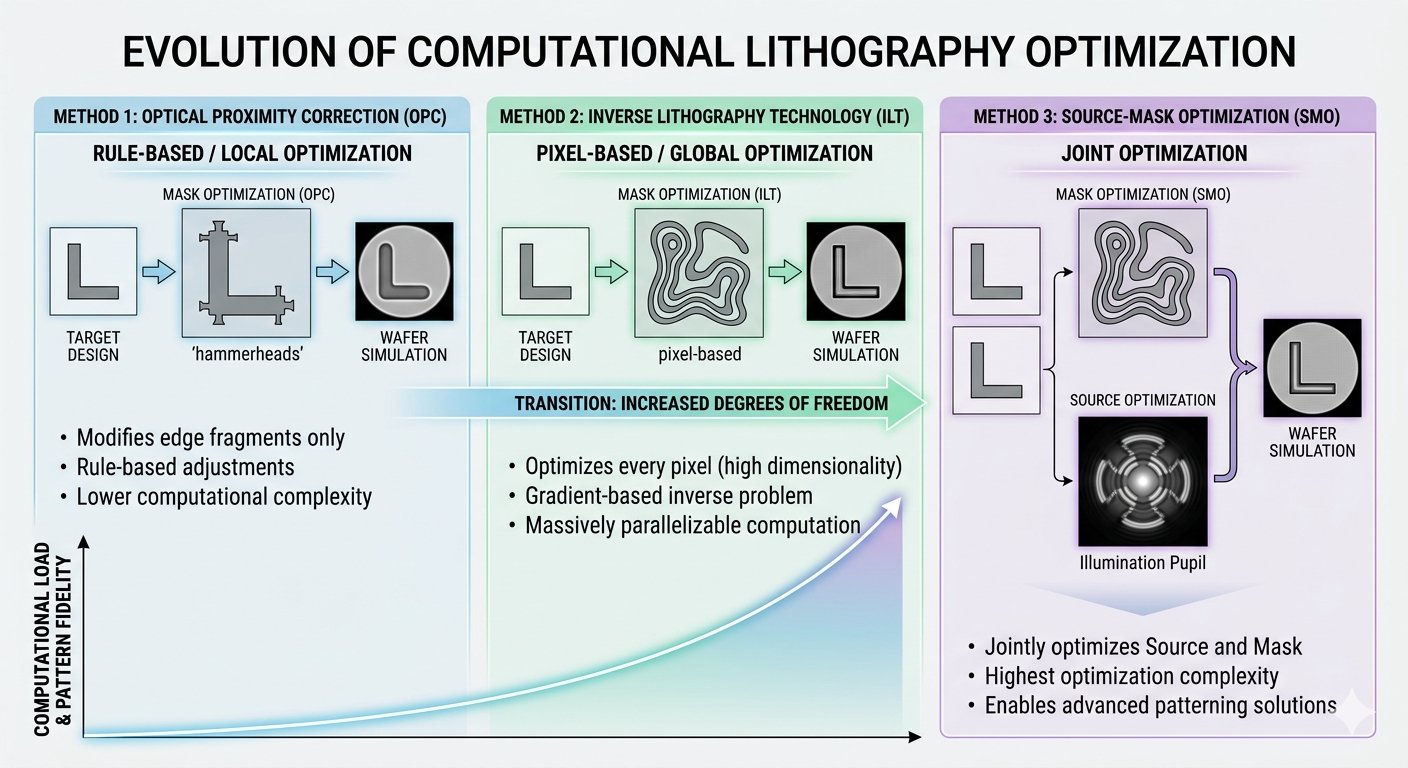
\includegraphics[width=1.0\linewidth]{images/lithography_Evolution.png}
  \caption{Lithography Techniques}
  \label{fig:Lithography Techniques}
\end{figure}


\subsection{Forward Lithography Models : The computational foundation}
One can think of forward lithography models as a feed-forward control system, which takes in mask as in input and predicts and final wafter pattern. These models serve as the inner loop of every optimization routine and are primary targets of GPU acceleration due to their data parallel structures. 

Forward lithography models predict the printed wafer pattern resulting from a given mask layout under specified optical and process conditions. These models form the computational backbone of OPC, ILT, and SMO workflows, as they must be evaluated repeatedly across large parameter spaces. In practice, forward models balance physical fidelity against computational tractability, with different formulations adopted depending on accuracy requirements and runtime constraints.

\begin{itemize}
  \item Fourier Optics and FFT : The most widely used class of forward models is based on Fourier optics, where aerial image computation is formulated as a convolution between the mask field and the optical system’s point spread function. In frequency space, this convolution reduces to elementwise multiplication, enabling efficient evaluation using FFTs on large spatial grids \cite{Mack2007FundamentalPO,Hopkins88,Wong2001ResolutionET}. 
  \item Partial Coherence : For partially coherent illumination, the forward model aggregates multiple independent Fourier-domain propagations corresponding to different source points or illumination modes, further increasing computational cost but improving predictive accuracy. Due to their regular structure and dense numerical operations, FFT-based forward models dominate runtime in many lithography simulation pipelines.
  \item Rigorous EM solvers: In situations where scalar diffraction models are insufficient—such as high numerical aperture imaging, strong mask topography effects, or extreme ultraviolet (EUV) lithography—rigorous electromagnetic (EM) solvers are employed. These solvers resolve Maxwell’s equations to capture vector effects, polarization, and three-dimensional mask interactions \cite{Wong2001ResolutionET}. While EM-based forward models provide higher fidelity, they are substantially more expensive than FFT-based approaches and are therefore typically used selectively, for example to calibrate reduced-order models or to analyze critical features rather than entire layouts.
\end{itemize}

A central consideration in forward lithography modeling is the tradeoff between accuracy and performance. FFT-based models enable rapid evaluation and are well suited for iterative optimization and full-chip analysis, but they rely on approximations that may miss subtle three-dimensional or polarization-dependent effects. EM solvers, by contrast, offer higher physical accuracy at the cost of orders-of-magnitude higher computational expense. Modern lithography workflows often combine these approaches, using EM simulations sparingly to inform or validate faster FFT-based models, thereby achieving an acceptable balance between predictive accuracy and computational scalability.

From a computational perspective, forward lithography models are well suited to parallel execution. FFT-based convolution, source decomposition, and pixel-level image formation all expose substantial data parallelism, enabling efficient acceleration on GPUs and GPU-accelerated clusters \cite{Govindaraju08,Zheng2023}. This parallel structure is a key reason forward models remain the primary targets for acceleration in both academic research and industrial lithography platforms, and it motivates the GPU-first design strategies discussed in subsequent sections.

\subsection{Inverse Formulations: From Heuristics to Massive Optimization}
Inverse lithography formulations seek to determine a mask pattern that produces a desired target pattern on the wafer under realistic optical and process conditions. This transition from prediction to 'sovling' has turned this into a feedback based control problem involving iterative gradient based optimizations. 

Unlike forward models, which evaluate a single mask configuration, inverse methods iteratively modify mask parameters to minimize discrepancies between simulated wafer images and design intent. This inversion is inherently ill-posed and high dimensional, as small changes in mask geometry can produce nonlocal and nonlinear effects in the printed pattern due to diffraction, partial coherence, and resist behavior \cite{Wong2001ResolutionET,cecil2022advances}.

There are 3 major techniques which fall in this category: 

\subsubsection{Optical Proximity Correction(OPC)}

Optical proximity correction (OPC) represents the earliest and most widely deployed inverse approach, traditionally operating on mask edges or fragments to compensate for systematic imaging distortions. While rule-based OPC relies on predefined heuristics, model-based OPC evaluates forward lithography models repeatedly to guide fragment adjustments \cite{capodieci2006optical}. Zheng et al. \cite{Zheng2024} explains the use of mathematical models to simulate image formation process and adjust the mask layout. It builds upon their previous work \cite{Zheng2023} about Open ILT to support model based OPC or MB OPC. They leverage GPU resources to accelerate the OPC computation, achieving significant speedup over the CPU based MB OPC method, while maintaining the same correction accuracy and quality.

OPC is an extensively used resolution enhancement technique (RET) in optical lithography . However, it's  computational efficiency has become a big issue for pixelated OPC techniques due to the increasing complexity of lithographic masks in modern integrated circuits. The dimensionality of the OPC problem is reduced by  downsampling the layout pattern. Then, a nonlinear cost function is established to guarantee the lithography imaging performance on the downsampled layout. 
Under the sparsity assumption of the mask, the OPC problem is formulated as an inverse nonlinear CS reconstruction problem.[\cite{ma2018fast},\cite{capodieci2006optical}]

In model  based OPC, masks are systematically modified to compensate for the nonideal optical and process effects of an optical lithography system. The polygons in the layout are fragmented, and simulations are performed to determine the image intensity pattern on the wafer. If the simulated pattern on the wafer does not match the desired one, the mask is perturbed by moving the fragments. This iterative process continues until the pattern on the wafer matches the desired one. Although OPC increases the fidelity of pattern transfer to the wafer, it is quite CPU intensive due to the simulations performed at each iteration. 

Linear regression techniques from statistical learning are used to predict the fragment movements. The goal is to reduce the number of iterations required in model based OPC by using a fast, computationally efficient linear regression solution as the initial guess to model based OPC. Experimental results show that fragment movement predictions via linear regression model significantly decrease the number of iterations required in model based OPC, thereby decreasing the product development time in IC design and manufacturing. [\cite{Gu2008}]


\subsubsection{Inverse Lithography Technology(ILT)}

\textcolor{blue}{ ILT is an approach used to calculate shapes of the photo masks which will produce exact desired pattern on the silicon wafer. ILT based approaches are computationally scalable, especially as they avoid laborious segmentation script writing, which becomes increasingly complex for newwer generations due to complicated proximity effects. ILT also benefits with simulation results and wafer examples and the impact of ILT in every step of mask making process. There are also studies done together with leading mask shops around the world on mask manufacturability with ILT (including data fracturing, writing strategy and writing time, mask inspection). \cite{pang2006inverse}}

Inverse lithography technology (ILT) formulates mask synthesis as a continuous or pixel-based optimization problem, allowing more degrees of freedom and improved pattern fidelity at advanced nodes \cite{cecil2022advances}. 

\textcolor{blue}{ Neural network based inverse lithography technology (NNILT) has been used to improve the computational efficiency of large scale mask optimization for advanced photolithography. NNILT is now mostly based on labels, and its performance is affected by the quality of labels. It is difficult for NNILT to achieve high performance and extrapolation ability for mask optimization without using labels. There are label free NNILT techniques(LF NNILT), which are implemented completely without labels and greatly improves the printability of the target layouts and the manufacturability of the synthesized masks compared to the traditional ILT. More importantly, the optimization speed of LF NNILT is two orders of magnitude faster than the traditional ILT. Furthermore, LF NNILT is simpler to implement and can achieve better solvers to support the development of advanced lithography.\cite{chen2022label}}

In lithography, optical proximity and process bias/effects need to be corrected to achieve the best wafer print \cite{pang2021inverse}. 
Efforts to correct for these effects started with a simple bias, adding a hammer head in line ends to prevent line end shortening. 
This first generation correction was called rule based optical proximity correction (OPC). Then, as chip feature sizes continued to shrink, 
OPC became more complicated and evolved to a model based approach. Some extra patterns were added to masks, to improve the wafer process window,
a measure of resilience to manufacturing variation. Around this time, the concept of ILT, a mathematically rigorous
inverse approach that determines the mask shapes that will produce the desired on wafer results, was introduced. ILT has been explored and developed 
over the last three decades as the next generation of OPC, promising a solution to several challenges of advanced node lithography, whether optical or 
extreme ultraviolet (EUV). Today, both OPC and ILT are part of an arsenal of lithography technologies called resolution enhancement technologies. 
Since OPC and ILT both involve computation, they are also considered as part of computational lithography. We explore the background and history of 
ILT and detail the significant milestones that have taken full chip ILT from an academic concept to a practical production reality.

Most inverse lithography approaches rely on gradient-based optimization. Gradients of the objective function with respect to mask parameters are obtained either through adjoint methods or approximate sensitivity analysis, enabling efficient updates even in large parameter spaces. These gradients must be evaluated repeatedly across thousands of iterations, with each iteration invoking one or more forward lithography simulations. As a result, inverse workflows are dominated by repeated execution of FFT-based imaging, resist modeling, and error evaluation, making them orders of magnitude more expensive than single forward simulations.

Robust optimization further amplifies this cost. To ensure manufacturability, inverse solutions must remain stable across process windows spanning focus, dose, aberrations, and other sources of variability. Robust ILT and SMO formulations therefore optimize expected or worst-case error metrics over ensembles of process conditions rather than a single nominal case. This requirement multiplies the number of forward model evaluations per iteration and significantly increases memory and compute demands, particularly for full-chip layouts.

At scale, GPUs are not optional accelerators but enabling infrastructure for inverse lithography. The massive data parallelism exposed by pixel-level mask representations, FFT-based imaging, and gradient evaluation aligns naturally with GPU execution models. More importantly, inverse workflows benefit from keeping the entire optimization loop device-resident, avoiding costly CPU–GPU data transfers between iterations. GPU-accelerated frameworks have demonstrated that this design dramatically improves throughput, energy efficiency, and multi-GPU scalability, enabling inverse lithography to transition from academic prototypes to production-scale deployment.


As Moore’s law has marched forward, progressively shrinking chip designs at a consistent pace, the manufacturing 
of those chips has raced to keep up. Through advances in lithography hardware and software, we now are in the realm of the single digit nanometer
design nodes at leading chip foundries. Cecil et al.\cite{cecil2022advances} reviews the method of ILT, which is the preferred computational
method for photolithography. Indeed photolithographic masks were the first metasurfaces, and still the most important metasurface, economically, 
used in memory chips, storage, and microprocessors. Moreover, photolithographic mask designers were the early adopters of the mathematical optimization
in optics, creating ILT, specifying intended wafer patterns and metrics, and using the mathematical machinery of level sets, functional derivatives, 
and adjoints to drive the mask design process.



\subsubsection{Source Mask Optimization(SMO)}
Source–mask optimization (SMO) further extends the inverse formulation by jointly optimizing illumination source parameters and mask geometry, increasing the dimensionality and computational complexity of the problem \cite{Socha66}.



In summary, OPC, ILT, and SMO recast lithography as large-scale inverse optimization problems whose computational intensity grows rapidly with layout complexity and process robustness requirements. Gradient-based methods and robust formulations make repeated forward simulation unavoidable, rendering inverse lithography fundamentally dependent on GPU acceleration and cluster-scale parallelism for practical use at advanced technology nodes. 


Figure 4 below show how these techniques continue to coexist to make advances in the field of lithography.

\begin{figure}[t]
  \centering
  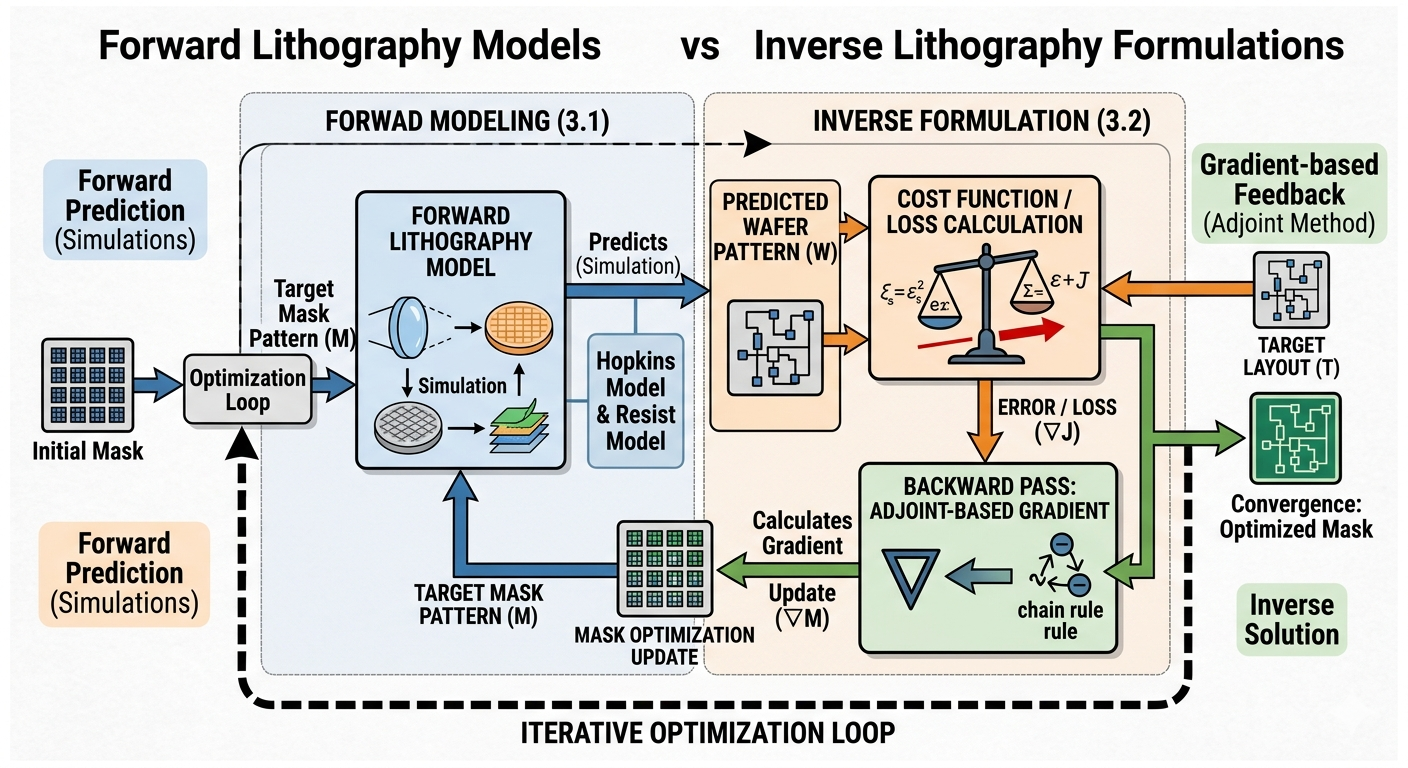
\includegraphics[width=1.0\linewidth]{images/computation.png}
  \caption{Forward vs Inverse Techniques}
  \label{fig:Forward vs Inverse Lithography}
\end{figure}





\section{GPU Architecture Considerations for Lithography}
\subsection{SIMT Execution and Parallel Structure} 
GPU acceleration of computational lithography relies critically on how lithography algorithms map onto the single-instruction, multiple-thread (SIMT) execution model. Unlike control-heavy workloads, lithography kernels are dominated by dense numerical operations over regular spatial grids, making them naturally compatible with SIMT execution when designed appropriately \cite{4490127,kirk10,navarro2014survey}. At a high level, pixel-level parallelism forms the foundation of this mapping: each image pixel, frequency-domain coefficient, or mask grid point can be processed independently across GPU threads, enabling large numbers of threads to execute identical operations concurrently.

This structure is particularly evident in optical imaging and resist simulation. FFT-based aerial image computation operates on uniform two-dimensional grids where each thread is responsible for updating one or more grid elements during forward and inverse transforms. Similarly, stencil-based resist solvers apply identical update rules across neighboring grid points, allowing thread blocks to process contiguous spatial regions with high utilization. These access patterns align well with SIMT execution because threads within a warp typically follow identical control paths and operate on adjacent memory locations, maximizing throughput and minimizing instruction divergence \cite{4490127,kirk10}.

However, efficient SIMT execution in lithography is not automatic and requires careful attention to kernel structure. Warp divergence can arise when conditional logic depends on spatially varying physical properties, such as thresholding operations in resist development, mask geometry irregularities, or region-specific correction rules in OPC. When threads within a warp take different execution paths, effective parallelism is reduced, leading to underutilization of GPU cores. Studies on GPU-accelerated lithography simulation have shown that naïvely ported kernels often suffer from such divergence, particularly in edge-based OPC routines, unless data layouts and control flow are explicitly reorganized to preserve warp coherence \cite{Zheng2023}.

FFT grid mapping also plays a central role in determining SIMT efficiency. Large FFTs are decomposed into multiple computation and data-reordering stages, each of which must be carefully mapped onto thread blocks to balance arithmetic intensity against memory access regularity. Well-structured FFT kernels expose fine-grained parallelism with predictable synchronization points, allowing SIMT execution to proceed with minimal divergence. GPU-accelerated lithography studies demonstrate that improper grid decomposition or misaligned data layouts can introduce irregular memory access and synchronization overhead that degrade performance, particularly at full-chip scales \cite{Zheng2023,Cao2023}.

From a systems perspective, SIMT efficiency directly impacts scalability and energy efficiency. High warp occupancy and low divergence enable forward and inverse lithography kernels to scale effectively across thousands of GPU cores and across multiple GPUs in a cluster. Conversely, divergence-heavy kernels limit achievable speedup and reduce performance per watt, undermining the benefits of GPU acceleration. As a result, modern GPU-accelerated lithography frameworks increasingly favor pixel-based and grid-based formulations over control-intensive approaches, structuring entire optimization pipelines to remain device-resident and SIMT-friendly \cite{Zheng2023,Cao2023}.

In summary, SIMT execution aligns well with lithography workloads due to their inherent pixel-level parallelism and grid-based numerical structure. Achieving high performance requires careful kernel design that maps FFT grids and resist stencils cleanly onto warps while minimizing divergence introduced by conditional logic. These considerations are fundamental to realizing scalable, energy-efficient GPU acceleration in computational lithography.

\subsection{Memory Hierarchy and Data Movement}
Memory behavior is a dominant performance and energy-efficiency factor in GPU-accelerated computational lithography. Unlike compute-bound kernels with minimal data reuse, lithography workloads repeatedly access large, structured data sets—including mask grids, pupil functions, optical transfer functions, and resist state variables—across thousands of iterations. As a result, effective utilization of the GPU memory hierarchy is essential for sustaining high throughput and avoiding bandwidth bottlenecks \cite{4490127,kirk10}.

FFT-based optical simulation is particularly sensitive to memory access patterns. Large two-dimensional FFTs require multiple passes over dense grids, interleaving computation with global memory reads, writes, and data reordering stages. When data are laid out contiguously and accessed in a coalesced manner, GPUs can exploit their high global memory bandwidth to achieve near-peak throughput. However, suboptimal layouts or frequent data transpositions can significantly degrade performance by increasing memory traffic and cache misses \cite{4490127,kirk10}. \textcolor{blue} {Owens et al.} highlight that full-chip lithography simulations often become memory-bandwidth bound rather than compute-bound, especially when operating on large frequency-domain grids.

Resist modeling introduces additional memory pressure. Reaction–diffusion solvers maintain multiple state variables per grid point and require repeated stencil-based updates that read from neighboring locations. While these access patterns exhibit spatial locality, their performance depends strongly on how intermediate fields are staged within the memory hierarchy. GPU-accelerated lithography studies show that retaining frequently accessed resist fields in on-device memory across iterations substantially reduces global memory traffic and improves overall efficiency \cite{Zheng2023}.

Data movement between the host and device represents one of the most significant sources of overhead in early GPU-based lithography implementations. Initial approaches often transferred intermediate results—such as aerial images or resist profiles—back to the CPU between simulation stages or optimization iterations. These transfers incur high latency and energy cost, quickly offsetting computational gains from GPU acceleration \cite{4490127}. More recent frameworks emphasize minimizing host–device communication by keeping the entire lithography pipeline device-resident, including optical simulation, resist modeling, and inverse optimization loops \cite{Zheng2023,Cao2023}.

Multi-GPU and cluster-scale execution further amplify the importance of data movement. When lithography domains are partitioned spatially or spectrally across GPUs, inter-device communication must be carefully managed to avoid synchronization bottlenecks. GPU-resident pipelines enable most communication to occur through high-bandwidth device interconnects rather than through the host, improving scalability and reducing contention on CPU memory subsystems \cite{Cao2023}. This design becomes increasingly important for robust ILT and SMO workflows, where multiple process conditions must be evaluated concurrently across GPUs.

From an energy-efficiency perspective, data movement is often more expensive than arithmetic operations. Excessive global memory access or host–device transfers can dominate power consumption, particularly in large-scale cluster deployments. By structuring lithography kernels to maximize data reuse within device memory and minimize unnecessary transfers, GPU-accelerated systems achieve higher performance per watt and better scalability under power constraints \cite{kirk10,Cao2023}.

In summary, effective management of the GPU memory hierarchy is critical for lithography workloads, which are characterized by large data sets, repeated access patterns, and tight coupling between simulation stages. Designs that emphasize coalesced memory access, device-resident data structures, and minimized host–device communication consistently outperform naïve GPU ports. These memory-centric considerations are therefore central to achieving scalable, energy-efficient computational lithography on modern GPU-accelerated clusters.

\subsection{Programming Models}
The choice of programming model plays a central role in determining the performance, portability, and maintainability of GPU-accelerated computational lithography systems. Lithography workloads are long-lived, performance-critical, and tightly integrated with industrial EDA flows, making ecosystem maturity and tooling support as important as raw computational capability  \cite{4490127,kirk10}. Consequently, programming model decisions in lithography are driven by practical deployment considerations in addition to theoretical performance.

In industrial practice, CUDA has emerged as the dominant programming model for GPU-accelerated lithography. Its adoption is driven by mature compiler support, highly optimized libraries for FFTs and linear algebra, and fine-grained control over memory hierarchy and execution behavior—capabilities that are essential for FFT-heavy optical simulation and tightly coupled inverse optimization loops  \cite{kirk10,Zheng2023}. While OpenCL provides portability across heterogeneous devices, its comparatively limited ecosystem, weaker tooling, and lack of vendor-optimized lithography-specific libraries have constrained its adoption in production environments. As emphasized in recent industrial platforms such as NVIDIA cuLitho, performance predictability and access to optimized CUDA libraries are critical factors for large-scale deployment \cite{Singh}.

The emergence of learning-assisted lithography has further influenced programming model choices. Neural-network-based inverse lithography (NN-ILT) frameworks use deep learning models to approximate or augment physics-based solvers, reducing the number of expensive forward simulations required during optimization. PyTorch has become the de facto framework for NN-ILT due to its automatic differentiation capabilities, flexible model composition, and seamless integration with CUDA \cite{jiang2021neural,Zhang2020}. This enables hybrid pipelines in which neural surrogates, gradient computation, and physics-based lithography kernels execute on the GPU within a unified programming environment, preserving device residency across optimization iterations.

Multi-GPU execution introduces additional programming challenges that directly affect scalability. Lithography workloads are typically decomposed using spatial tiling of the mask or spectral partitioning of optical computations, allowing independent subproblems to be distributed across GPUs \cite{Zheng2023,yang2024gpuacceleratedinverselithographyhigh}. Programming models must support efficient orchestration of these tiles while minimizing synchronization and communication overhead. CUDA-based frameworks provide explicit mechanisms for multi-GPU coordination and peer-to-peer communication, enabling scalable implementations on GPU clusters. By contrast, higher-level abstractions that obscure data movement often limit the ability to optimize performance-critical lithography kernels at scale \cite{yang2024gpuacceleratedinverselithographyhigh}.

From a software engineering perspective, modern lithography systems increasingly adopt hybrid programming models. Performance-critical kernels are implemented in CUDA to maximize efficiency, while higher-level frameworks such as PyTorch \cite{paszke2019pytorch} support rapid prototyping, algorithm development, and integration of learning-based components. Document B highlights that this layered approach has become common in both academic research and industrial platforms, balancing productivity with the stringent performance requirements of computational lithography.

In summary, programming models for GPU-accelerated computational lithography reflect a pragmatic balance between performance, ecosystem maturity, and extensibility. CUDA dominates industrial deployments due to its optimized libraries and tooling support, PyTorch enables effective integration of neural inverse methods, and explicit multi-GPU tiling strategies remain essential for scaling lithography workloads on cluster architectures.

\begin{figure}[b]
  \centering
  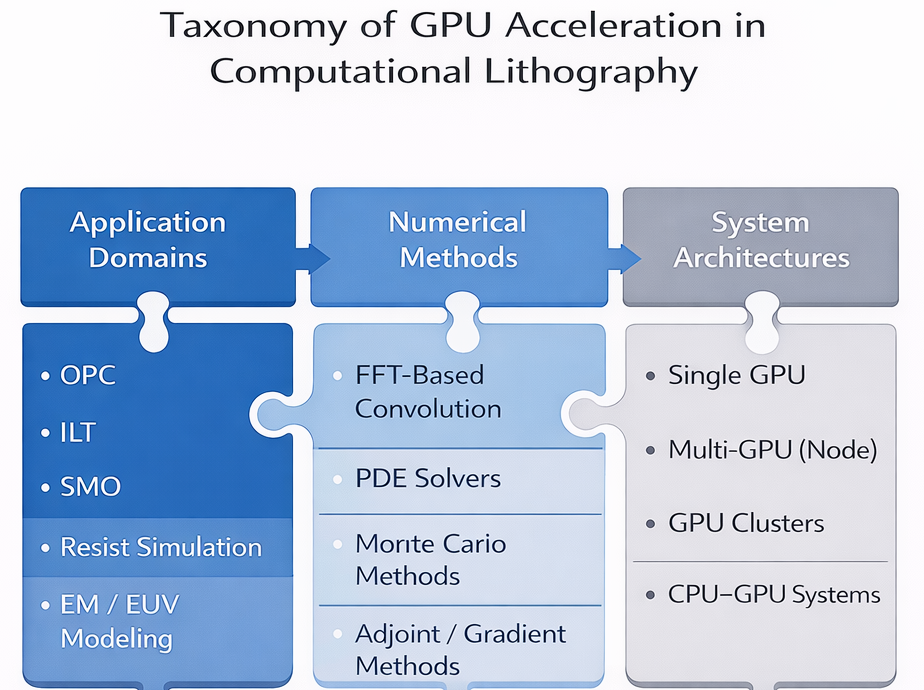
\includegraphics[width=0.7\linewidth]{images/fig2.png}
  \caption{Taxonomy of GPU acceleration in computational lithography, organized across application domains, numerical methods, and system architectures.}
  \label{fig:taxonomy}
\end{figure}

\section{Taxonomy of GPU Acceleration in Computational Lithography}
To systematically organize prior work on GPU-accelerated computational lithography, this section introduces a taxonomy spanning three complementary dimensions: application domains, numerical methods, and system architectures. This taxonomy provides a unified perspective on how GPU acceleration is employed across lithography workflows and clarifies why different computational and architectural strategies are required in practice. Figure \ref{fig:taxonomy} summarizes this taxonomy and serves as a roadmap for the discussion in the remainder of this section.




\subsection{Application-Level Taxonomy}
GPU acceleration in computational lithography spans a diverse set of applications that differ significantly in computational structure, accuracy requirements, and scalability demands. An application-level taxonomy provides a unifying view of how GPUs are employed across lithography workflows and clarifies why different acceleration strategies are required in practice \cite{cecil2022advances,Wong2001ResolutionET}. We categorize prior work into five primary application classes: OPC, ILT, SMO, resist simulation, and EM/EUV modeling.

\subsubsection{Optical Proximity Correction (OPC)}
Optical Proximity Correction (OPC) is the most mature and widely deployed application of computational lithography and a core component of resolution enhancement techniques (RET) used in modern semiconductor manufacturing \cite{subramany2011gpu}. Model-based OPC iteratively modifies mask edges or fragments to compensate for diffraction-limited imaging and process effects that arise from the mismatch between the exposure wavelength and the target feature dimensions. Each correction step requires forward lithography simulation to evaluate the impact of mask modifications on the printed wafer pattern, making simulation throughput a primary determinant of overall OPC runtime.

The computational cost of OPC is dominated by repeated FFT-based optical imaging evaluated across many correction iterations and layout contexts. GPU acceleration in OPC therefore focuses on pixel-level aerial image computation and error evaluation, where dense grid operations and limited control divergence enable high SIMT efficiency. While early OPC implementations offloaded only isolated imaging kernels to GPUs, more recent systems increasingly favor GPU-resident pipelines that minimize host–device data movement and improve throughput at full-chip scale \cite{Zheng2023}. As a result, fast and scalable lithography simulation is essential for practical OPC deployment, particularly when applied to advanced technology nodes and large layouts.

\subsubsection{Inverse Lithography Technology (ILT)}
Inverse Lithography Technology (ILT) generalizes OPC by formulating mask synthesis as a large-scale inverse optimization problem with pixel-level or curvilinear degrees of freedom \cite{Gallatin2005}. Compared to OPC, ILT exposes substantially higher computational intensity due to continuous optimization variables, gradient computation, and the need for thousands of iterative updates. ILT workflows are therefore dominated by repeated execution of forward imaging and resist models within gradient-based or adjoint optimization loops, making computational efficiency a first-order concern \cite{Gallatin2005,smith2003methods}.

Because ILT solutions must be optimized not only for pattern fidelity but also for manufacturability and robustness across process windows, inverse optimization is typically performed over ensembles of exposure, focus, and process conditions. This requirement further multiplies the number of forward simulations required per iteration. GPUs are particularly effective for ILT because pixel-based mask representations, FFT-heavy imaging, resist evaluation, and gradient computation all map naturally to data-parallel execution. As a result, ILT has emerged as one of the primary drivers for GPU-first and multi-GPU lithography systems in both academic frameworks and industrial platforms such as OpenILT and NVIDIA cuLitho \cite{torunoglu2010gpu,Singh}.


\subsubsection{Source–Mask Optimization (SMO)}
Sfurther extends inverse lithography by jointly optimizing illumination source parameters and mask geometry within a unified inverse formulation \cite{Socha66}. By coupling source and mask degrees of freedom, SMO significantly increases problem dimensionality relative to ILT, as each optimization step must evaluate multiple illumination configurations in addition to mask updates. This coupling introduces strong interactions between optical conditions and mask features, requiring repeated forward lithography simulations to accurately capture imaging behavior across the combined design space.

From a computational perspective, SMO is particularly demanding because robustness considerations require evaluating ensembles of source–mask configurations over process windows that include focus, dose, and aberration variations. As a result, the cost of a single SMO iteration can exceed that of ILT by an order of magnitude, making brute-force or CPU-only approaches impractical at full-chip scale. GPU acceleration is therefore essential for SMO, as it enables efficient parallelization of source decomposition, FFT-based multi-condition imaging, and error aggregation across illumination modes.

GPUs are commonly used to exploit parallelism across independent source points and spatial domains, allowing thousands of optical simulations to be evaluated concurrently. At larger scales, multi-GPU systems further enhance throughput by distributing independent source–mask evaluations across devices, reducing synchronization overhead and enabling strong scaling. This natural decomposition makes SMO a strong candidate for cluster-scale execution, where GPU-accelerated nodes can be orchestrated to explore high-dimensional optimization spaces efficiently. Consequently, SMO exemplifies a class of lithography applications in which GPU acceleration is not merely beneficial but fundamentally enabling.

\subsubsection{Photoresist Simulation}
Photoresist simulation translates aerial images into final wafer patterns and associated variability metrics by modeling the underlying photochemical reactions and development processes within the resist. These models are essential for predicting critical dimension variations, line-edge roughness, and stochastic printing failures that increasingly limit yield at advanced technology nodes. As discussed in Document A, resist modeling is computationally demanding due to the use of stencil-based reaction–diffusion solvers and stochastic Monte Carlo simulations, particularly in extreme ultraviolet (EUV) lithography where low photon counts lead to significant shot noise effects \cite{Gallatin2005,Mack2007FundamentalPO}.

From a computational perspective, resist simulation introduces both high arithmetic intensity and substantial memory pressure. Reaction–diffusion models require repeated updates over dense spatial grids, while Monte Carlo approaches demand large numbers of statistically independent samples to obtain stable variability estimates. GPU acceleration in this category exploits strong spatial locality and massive parallelism across grid points or stochastic samples, enabling efficient evaluation of variability metrics that would otherwise be prohibitive on CPU-based systems. These characteristics make resist simulation particularly well suited to SIMT execution and multi-GPU scaling.

Resist modeling is often invoked not only as a standalone analysis tool but also as a tightly coupled component within OPC and ILT workflows, where it must be evaluated repeatedly across optimization iterations and process conditions. In such settings, retaining resist state variables and intermediate fields in device memory is critical for minimizing data movement overhead and sustaining throughput. GPU-resident execution has therefore become a key design principle for scalable resist simulation, especially when integrated into inverse lithography pipelines that require thousands of resist evaluations \cite{Zheng2023}.

\subsubsection{Electromagnetic (EM) and Extreme UltraViolet (EUV) Modeling}
Rigorous electromagnetic simulation becomes necessary when scalar diffraction models are no longer sufficient, such as in high–numerical-aperture (high-NA) and extreme ultraviolet (EUV) lithography, where vector effects, polarization, shadowing, and three-dimensional mask topography significantly influence image formation and pattern fidelity \cite{Wong2001ResolutionET,2017JMM&M}. In these regimes, EM solvers resolve Maxwell’s equations to accurately capture near-field interactions and mask-induced effects that cannot be represented by FFT-based imaging models.

Despite their accuracy, EM-based lithography models are substantially more computationally expensive than scalar optical simulations. They involve large-scale field updates, dense linear algebra, and fine spatial discretization, leading to high memory footprints and long runtimes. Consequently, EM solvers are typically applied selectively in practice—for example, to analyze critical features, validate simplified optical models, or calibrate reduced-order representations used in full-chip simulation flows \cite{shamoun2021multi}. This selective use reflects a pragmatic balance between physical fidelity and computational feasibility.

GPU acceleration in EM and EUV modeling primarily targets dense numerical kernels such as field propagation, matrix operations, and domain-decomposed updates. While GPUs can provide significant speedups for these kernels, scalability is often constrained by memory capacity, irregular data access patterns, and inter-device communication overhead, particularly in three-dimensional simulations. As a result, EM and EUV lithography modeling commonly adopts hybrid strategies that combine GPU acceleration with hierarchical modeling, domain decomposition, or reduced-order techniques. These approaches leverage GPUs where they are most effective while mitigating scalability limitations, enabling EM accuracy to be incorporated into larger lithography workflows without incurring prohibitive computational cost.

\subsubsection{Summary}
This application-level taxonomy highlights that GPU acceleration in computational lithography is inherently heterogeneous. OPC emphasizes high-throughput imaging, ILT and SMO demand large-scale inverse optimization, resist simulation stresses stochastic and stencil-based computation, and EM/EUV modeling prioritizes physical fidelity over throughput. These distinctions motivate different numerical methods and system architectures, which are formalized in the following taxonomy levels.


\subsection{Numerical Method Taxonomy}
Beyond application-level distinctions, GPU acceleration strategies in computational lithography can be categorized by the underlying numerical methods they accelerate. Each method exhibits distinct computational patterns, memory behaviors, and scalability characteristics that strongly influence how effectively it maps onto GPU architectures. We classify prior work into four primary numerical categories: FFT-based convolution, PDE solvers, Monte Carlo methods, and adjoint-based optimization.
\subsubsection{FFT-Based Convolution}
FFT-based convolution forms the computational core of scalar optical imaging models used in OPC, ILT, and SMO workflows. In these formulations, aerial image computation is expressed as a convolution between the mask field and the optical system response, which is efficiently evaluated in the frequency domain using FFTs \cite{Hopkins88,Mack2007FundamentalPO}. Because partial coherence and multi-condition imaging require repeated FFT evaluations across illumination modes, focus values, and optimization iterations, FFT-based methods often dominate runtime in lithography simulation \cite{Wong2001ResolutionET}. These dense, regular grid operations exhibit high arithmetic intensity and predictable memory access patterns, making FFT acceleration one of the most mature and effective uses of GPUs in computational lithography \cite{Zheng2023}.

\subsubsection{Partial Differential Equation (PDE) Solvers}
PDE-based methods arise primarily in photoresist modeling, where reaction–diffusion equations describe the generation, transport, and amplification of chemical species during exposure and development \cite{NEUREUTHER1992377}. These solvers typically employ stencil-based updates over fine spatial grids and require repeated time stepping, leading to substantial computational cost. From a numerical standpoint, PDE solvers exhibit strong spatial locality and uniform control flow, which align well with SIMT execution on GPUs. However, performance is often limited by memory bandwidth rather than compute throughput, particularly for three-dimensional resist models \cite{Mack2007FundamentalPO}. GPU acceleration in this category focuses on optimizing stencil operations and maximizing data reuse across iterations \cite{yang2024gpuacceleratedinverselithographyhigh}.

\subsubsection{Monte Carlo Methods}
Monte Carlo methods play a central role in computational lithography when modeling stochastic physical phenomena that cannot be accurately captured by deterministic formulations. In particular, resist simulation for extreme ultraviolet (EUV) lithography relies heavily on Monte Carlo techniques to account for photon shot noise, secondary electron generation, and chemical reaction variability. These stochastic effects are a primary source of line-edge roughness and critical dimension variation, making Monte Carlo modeling essential for yield-aware lithography analysis.

From an algorithmic perspective, Monte Carlo resist modeling relies on parallel random number generation to support large ensembles of independent stochastic samples and spatial grid points. Efficient generation and management of statistically independent random streams is therefore a critical requirement for scalable simulation, especially on massively parallel architectures \cite{LEcuyer2015}. GPU-accelerated Monte Carlo simulations are widely used in stochastic physical modeling, as their embarrassingly parallel structure maps naturally to thousands of concurrent threads \cite{Sakane2022}.

The application of Monte Carlo techniques to physical simulation predates modern lithography and has been extensively studied in broader computational physics contexts. Early Monte Carlo simulations of carrier transport and noise phenomena in semiconductor materials provide historical grounding for contemporary resist modeling approaches \cite{Gruzinskis2008}. Modern lithography workflows build upon these foundations while extending them to significantly larger problem sizes and tighter accuracy requirements.

In practice, GPU acceleration enables Monte Carlo resist simulations that would otherwise be computationally prohibitive on CPU-based systems. However, scalability is often constrained by random number quality, memory bandwidth, and synchronization overhead when aggregating statistical metrics. As a result, continued advances in parallel random number generation, memory-efficient sampling strategies, and multi-GPU execution remain critical research directions for stochastic lithography modeling.

\subsubsection{Adjoint and Gradient-Based Methods}
Adjoint methods underpin gradient-based optimization in ILT and SMO by enabling efficient computation of sensitivities with respect to large numbers of mask and source parameters \cite{cecil2022advances}. Rather than computing gradients independently for each parameter, adjoint formulations reuse forward simulation results to evaluate gradients at a cost comparable to a small number of forward solves. Numerically, adjoint computations reuse many of the same kernels as forward models, including FFT-based imaging and resist evaluation, but with reversed data flow and accumulation steps \cite{yang2024gpuacceleratedinverselithographyhigh}. GPU acceleration is essential in this category because gradients must be evaluated repeatedly across thousands of optimization iterations and process conditions. Efficient adjoint implementations rely on GPU-resident execution to minimize data movement and sustain throughput in large-scale inverse lithography workflows \cite{Zheng2024}.

\subsubsection{Summary}
This numerical method taxonomy highlights that GPU acceleration in computational lithography targets a diverse set of computational patterns, ranging from dense FFTs and stencil-based PDE solvers to embarrassingly parallel Monte Carlo sampling and tightly coupled adjoint computations. Understanding these numerical characteristics is critical for selecting appropriate GPU programming models and system architectures, which we formalize in the following system-level taxonomy.


\subsection{System-Level Taxonomy}
At the system level, GPU acceleration in computational lithography spans a range of deployment configurations that reflect increasing problem scale, robustness requirements, and integration complexity. These configurations differ in how computation and data are partitioned across devices and how tightly GPU execution is coupled to the overall lithography workflow. We classify prior work into four system-level categories: single-GPU systems, multi-GPU systems, GPU clusters, and heterogeneous CPU–GPU systems.

\subsubsection{Single-GPU Systems}
Single-GPU configurations represent the earliest and simplest deployment model for GPU-accelerated lithography. In this setting, individual kernels—most commonly FFT-based optical imaging or localized resist evaluation—are offloaded to a single device while the remainder of the workflow executes on the CPU \cite{ZHANG2015176}. Early GPU-accelerated lithography studies demonstrated substantial speedups for aerial image computation and small-scale OPC tasks using this model, making it attractive for prototyping and limited-layout analysis. However, single-GPU systems are constrained by device memory capacity and cannot efficiently support full-chip ILT or SMO workflows that require evaluating large layouts across many process conditions \cite{yang2024gpuacceleratedinverselithographyhigh}.


\subsubsection{Multi-GPU Systems}
Multi-GPU systems extend single-device acceleration by distributing computation across multiple GPUs within a node or tightly coupled system. In computational lithography, this approach is commonly used to partition spatial domains, illumination source components, or independent process conditions across devices. Multi-GPU implementations of ILT and SMO exploit the independence of forward simulations and gradient evaluations to reduce iteration time and improve throughput. While this configuration enables larger problem sizes and higher performance, its efficiency depends on careful management of inter-device communication and synchronization, particularly when shared data such as mask updates or resist state variables must be exchanged \cite{Zheng2023}.

\subsubsection{GPU Clusters}
GPU clusters represent the most scalable system configuration and are increasingly required for production-scale ILT, SMO, and robust optimization workflows. In this model, lithography computations are distributed across many GPU-equipped nodes, enabling concurrent evaluation of large ensembles of process conditions, illumination settings, or optimization candidates \cite{Zheng2023}. Cluster-scale GPU acceleration is especially effective for SMO and robust ILT, where independent simulations dominate runtime and communication overhead can be minimized through embarrassingly parallel decomposition. Recent industrial platforms, such as NVIDIA’s cuLitho, exemplify this trend by leveraging GPU clusters to achieve order-of-magnitude reductions in turnaround time for full-chip lithography optimization \cite{Singh}.

\subsubsection{Heterogeneous CPU–GPU Systems}
Heterogeneous CPU–GPU systems combine the strengths of both architectures by assigning compute-intensive numerical kernels to GPUs while retaining control logic, optimization orchestration, and irregular tasks on CPUs. This configuration remains common in industrial lithography flows due to legacy software integration and tight coupling with existing EDA infrastructure. In many reported systems, CPUs manage scheduling, convergence checks, and I/O, while GPUs execute FFT-based imaging, resist simulation, and gradient evaluation \cite{yang2024gpuacceleratedinverselithographyhigh}. Although recent designs increasingly push toward GPU-resident execution of entire pipelines to reduce host–device communication overhead, heterogeneous systems continue to play an important role in transitional and hybrid deployments \cite{Zheng2023}.


\subsubsection{Summary}
This system-level taxonomy illustrates how GPU acceleration in computational lithography evolves from isolated kernel offloading toward fully GPU-resident, cluster-scale execution as problem size and robustness requirements increase. Single-GPU systems enable early acceleration, multi-GPU systems address memory and throughput limitations, GPU clusters unlock large-scale inverse optimization, and heterogeneous CPU–GPU systems balance performance with practical integration constraints.


\section{Frameworks, Tools, and Industrial Adoption}
The maturation of GPU acceleration in computational lithography has led to the emergence of both industrial-strength platforms and academic research frameworks. While these systems differ in scope, licensing, and deployment environments, they share common architectural principles shaped by the extreme computational demands of modern lithography. Prior studies consistently show that system-level design choices—rather than isolated kernel optimizations—largely determine scalability and energy efficiency in practice \cite{yang2024gpuacceleratedinverselithographyhigh,Zheng2023}.

\subsection{Timeline of Developments}
The evolution of GPU acceleration in computational lithography has progressed through several distinct phases, reflecting advances in GPU hardware, numerical algorithms, and system-level integration. This timeline highlights key developments that shaped the transition from early academic exploration to large-scale industrial adoption.
\begin{itemize}
  \item \textbf{2005 - 2015 Early Academic Exploration of GPU-Accelerated FFTs}: The initial phase of GPU adoption in computational lithography focused on accelerating FFT-based optical simulations. Academic studies during this period demonstrated that GPUs could significantly outperform CPUs for large-scale Fourier-domain imaging, establishing the feasibility of GPU acceleration for core lithography kernels. These early efforts primarily targeted standalone optical simulations and proof-of-concept acceleration rather than full lithography workflows.
  \item \textbf{2015 - 2018 Emergence of OpenILT and Experimental GPU Acceleration}: The introduction of research platforms such as OpenILT marked a shift toward system-level experimentation with GPU-accelerated inverse lithography. During this period, GPUs were increasingly used to accelerate not only optical imaging but also optimization loops and gradient computation. Although these efforts demonstrated strong scalability potential, GPU acceleration remained largely confined to academic and experimental settings, with limited penetration into production EDA tools.
  \textcolor{blue}{\item  \textbf{2019 - Introduction of TruMask ILT by D2S Inc.}: The introduction of curvilinear ILT tools enabled efficient synthesis of advanced mask geometries required at state-of-the-art nodes. These developments signaled a shift toward GPU-first architectures designed explicitly for large-scale inverse optimization and cluster execution, rather than incremental acceleration of legacy flows.  D2S Inc. introduced TruMask ILT; a novel sitchless approach to reduce curvilinear ILT timing from weeks to a day.}
  \item \textbf{2020 - 2023 Initial GPU Integration in Commercial Tools}: Between 2020 and 2023, major commercial lithography tools—including Synopsys S-Litho—began integrating GPU support for selected computational modules. This phase represented a transitional period in which GPU acceleration moved from research prototypes into production environments. However, most deployments adopted hybrid CPU–GPU architectures, accelerating isolated kernels while retaining CPU-centric workflow control.
  \item \textbf{2023 - 2025 NVIDIA cuLitho}: The launch of NVIDIA cuLitho marked a significant inflection point by demonstrating a fully GPU-resident lithography pipeline capable of delivering up to 40× speedups over traditional CPU-based flows. 
\end{itemize}

\subsection{Industrial Platforms}
Industrial lithography platforms prioritize robustness, predictability, and tight integration with existing electronic design automation (EDA) flows. GPU acceleration in production environments is therefore characterized by carefully engineered pipelines, optimized numerical libraries, and an emphasis on sustained throughput rather than peak kernel performance.

\subsubsection{NVIDIA cuLitho}
NVIDIA’s cuLitho platform represents a GPU-first redesign of computational lithography for production-scale deployment \cite{Singh}. Rather than accelerating isolated kernels, cuLitho integrates optical simulation, resist modeling, and inverse optimization into a unified, GPU-resident pipeline. By leveraging optimized FFT libraries, custom CUDA kernels, and device-resident data structures, cuLitho reports order-of-magnitude improvements in runtime and energy efficiency compared to CPU-based lithography flows. An important architectural lesson demonstrated by cuLitho is that end-to-end GPU residency—rather than incremental kernel offloading—is essential for scaling ILT and SMO workloads that require thousands of tightly coupled iterations.

\subsubsection{Synopsys S-Litho}
Synopsys S-Litho is a widely deployed industrial lithography simulation platform that has progressively incorporated GPU acceleration into its workflow to address the growing computational demands of advanced patterning \cite{SynopsysSLitho}. Originally designed around CPU-based execution, S-Litho integrates GPUs primarily to accelerate compute-intensive components such as FFT-based optical imaging and selected resist calculations. This hybrid CPU–GPU approach delivers meaningful performance gains while preserving compatibility with established electronic design automation (EDA) flows. At the same time, it illustrates a limitation observed across several hybrid architectures: frequent CPU–GPU data transfers and fragmented acceleration can constrain scalability and reduce achievable speedup at large problem sizes. As such, S-Litho exemplifies a transitional system architecture that balances legacy integration with incremental GPU adoption.

From a modeling perspective, S-Litho supports a broad range of lithographic patterning technologies, including proximity printing, deep ultraviolet (DUV), extreme ultraviolet (EUV), and electron-beam lithography. It enables detailed analysis of process-limiting effects within exposure systems by accounting for optical imaging, mask and substrate topography, and photoresist interactions. Integration with technology computer-aided design (TCAD) tools, such as Sentaurus Topography, allows coupled simulation of lithography and downstream process steps, supporting advanced integration techniques including multiple patterning. In addition, tight coupling with mask synthesis and verification tools facilitates model-based OPC development and automated hotspot analysis, reducing verification turnaround time.

At a system level, S-Litho demonstrates how comprehensive modeling capability and industrial robustness can coexist with selective GPU acceleration. While its modular design enables targeted performance improvements, it also highlights why emerging GPU-first platforms increasingly favor deeper pipeline integration and device-resident execution. These contrasting approaches underscore an important architectural lesson for scalable computational lithography: sustained performance gains require not only fast numerical kernels, but also careful coordination of data movement, control flow, and system-level design.

\subsubsection{Curvilinear ILT Tools}
Curvilinear ILT tools represent a growing class of industrial and near-industrial solutions that exploit continuous or curve-based mask representations to improve pattern fidelity at advanced technology nodes, particularly where Manhattan geometries are insufficient to compensate for diffraction and process effects \cite{cecil2022advances}. By allowing mask features to evolve smoothly rather than through discrete edge fragments, curvilinear ILT enables improved edge placement accuracy and process window robustness, but at the cost of substantially increased computational complexity.

Several representative tools and frameworks illustrate this trend. Early industrial and academic ILT implementations introduced pixel-based and curvilinear mask parameterizations to enable continuous optimization of mask shapes, demonstrating improved fidelity relative to traditional OPC approaches \cite{Socha66,cecil2022advances}. More recent production-oriented systems, including GPU-accelerated ILT engines integrated into commercial lithography platforms, extend these ideas to full-chip optimization using dense mask representations and gradient-based solvers. NVIDIA’s cuLitho platform further highlights the viability of curvilinear and pixel-level ILT at scale by combining GPU-resident FFT-based imaging, adjoint gradient computation, and multi-condition robustness analysis within a unified GPU-first architecture \cite{Singh}.

From a computational standpoint, curvilinear ILT tools are inherently demanding. They rely on large-scale inverse optimization with millions of continuous variables, repeated execution of forward lithography models, and evaluation across extensive process windows. GPU acceleration is therefore critical, particularly for FFT-heavy optical simulation, gradient and adjoint computation, and parallel evaluation of multiple exposure conditions. As these workloads scale beyond the capacity of single devices, curvilinear ILT tools increasingly adopt GPU-dominant and multi-GPU designs, reflecting a broader architectural shift toward systems capable of sustaining high iteration rates, large memory footprints, and cluster-scale execution \cite{Singh}.

\subsection{Academic and Open Frameworks}
Academic and open-source frameworks complement industrial tools by exploring new algorithms, optimization strategies, and architectural designs that may later influence production systems. These platforms typically emphasize flexibility and extensibility, making them valuable testbeds for evaluating scalability and performance tradeoffs.

\subsubsection{OpenILT}
OpenILT is a prominent open-source inverse lithography framework designed to support research on ILT algorithms and GPU acceleration strategies \cite{Zheng2023}. Its modular architecture decouples forward lithography simulation, resist modeling, optimization solvers, and evaluation metrics, enabling researchers to rapidly prototype and evaluate new algorithmic and architectural ideas. This modularity makes OpenILT particularly well suited for exploring tradeoffs between numerical methods, optimization strategies, and system-level designs.

A key contribution of OpenILT is its demonstration that full-pipeline GPU residency—where optical simulation, gradient computation, and optimization loops remain entirely on the device—significantly improves scalability compared to hybrid CPU–GPU designs, especially for gradient-based ILT workflows. By minimizing host–device data transfers and exposing fine-grained parallelism across pixels and process conditions, OpenILT enables sustained throughput over thousands of optimization iterations. At the same time, experiences with OpenILT highlight practical challenges that arise at scale, including memory footprint growth, synchronization overhead, and efficient orchestration across multiple GPUs or cluster nodes.

Overall, OpenILT serves as a valuable reference platform that illustrates both the potential and the limitations of GPU-centric ILT architectures. Its open design has influenced subsequent academic and industrial efforts by clarifying which architectural choices scale effectively and which introduce bottlenecks as problem size and robustness requirements increase.

\subsubsection{Learning-Based and Curvilinear ILT Frameworks}
Building on GPU-accelerated physics-based optimization, recent research has explored learning-based inverse lithography as a complementary approach for reducing computational cost. Neural-network-based ILT (Neural ILT) frameworks integrate deep learning models to approximate or augment traditional inverse optimization, leveraging GPUs for neural inference, automatic differentiation, and training \cite{jiang2021neural}. By predicting mask updates directly from layout features, Neural ILT approaches can significantly reduce turnaround time while maintaining competitive printability and mask complexity.

For example, Jiang et al. proposed an end-to-end Neural ILT framework in which a single neural network performs mask prediction and correction, targeting enhanced printability, reduced mask complexity, and accelerated optimization \cite{jiang2021neural}. Their results demonstrate substantial speedups relative to conventional ILT and prior learning-based OPC solutions, highlighting the potential of combining GPU-accelerated learning with lithography workflows. These approaches are most effective when neural surrogates are tightly integrated with GPU-resident physics models, enabling hybrid optimization loops that avoid excessive data movement.

In parallel, advances in curvilinear ILT have demonstrated the manufacturability benefits of continuous mask representations. Pang et al. introduced a stitchless, full-chip curvilinear ILT approach enabled by multi-beam mask writers, showing that curvilinear mask shapes can significantly improve robustness to manufacturing variation and substantially expand wafer process windows in memory chip fabrication \cite{pang2021breakthrough}. While curvilinear ILT imposes higher computational demands due to dense, continuous optimization variables, these studies provide strong empirical evidence that the added complexity is justified when supported by scalable GPU-based frameworks.

Together, learning-based and curvilinear ILT frameworks underscore a broader trend toward GPU-centric, hybrid optimization pipelines that combine physics-based models, data-driven surrogates, and large-scale parallel execution. These approaches reinforce the architectural lesson that future ILT systems must be designed holistically—integrating algorithms, data movement, and hardware—to achieve both performance and manufacturability at advanced technology nodes.

\subsection {Enabling Technical Innovations}
Beyond specific platforms and frameworks, several technical innovations have played a critical role in enabling scalable GPU acceleration for computational lithography. These advances span numerical kernels, optimization strategies, and data representations that collectively make modern lithography workloads tractable on GPU-based systems.
\subsubsection{GPU-Accelerated FFTs for Aerial Image Computation}
FFT-based optical imaging remains a dominant computational kernel in scalar lithography simulation and inverse optimization. Early work demonstrated that GPUs are particularly well suited for accelerating large-scale FFTs due to their high arithmetic throughput and memory bandwidth. Yu et al. presented GPU-based methods for accelerating mask optimization workflows by exploiting FFT parallelism, showing significant performance improvements over CPU implementations for aerial image computation \cite{YuZiyang2023}. These results reinforced the observation that FFT-heavy imaging pipelines naturally align with GPU architectures and can sustain high utilization when executed on dense grids.

GPU-accelerated FFTs now form the backbone of both academic and industrial lithography tools, underpinning OPC, ILT, and SMO workflows. Their efficiency is especially critical in inverse optimization, where optical simulations must be evaluated repeatedly across many iterations and process conditions. The widespread availability of optimized GPU FFT libraries has therefore been a key enabler for transitioning lithography simulation from isolated kernel acceleration to fully GPU-resident pipelines, as seen in modern platforms discussed earlier in Section 6.

\subsubsection{GPU-Accelerated ILT and Curvilinear Mask Generation}
The shift from traditional Manhattan mask geometries toward curvilinear representations has been driven by the need for higher pattern fidelity and improved process windows at advanced technology nodes. Choi et al. highlighted the growing importance of curvilinear masks for achieving high-quality wafer patterns, demonstrating their superior ability to compensate for diffraction and process effects compared to conventional OPC approaches \cite{Choi2021}. Related work has also emphasized the limitations of traditional OPC under focus variations and complex process conditions, further motivating the adoption of ILT-based solutions \cite{Yu2024}. Figure~\ref{fig:curvilinear_vs_manhattan} illustrates the fundamental geometric differences between Manhattan and Curvilinear mask representations and their impact on wafer pattern fidelity. However, curvilinear ILT significantly increases computational complexity due to dense, continuous optimization variables and repeated evaluation of forward lithography models.

\begin{figure}[t]
  \centering
  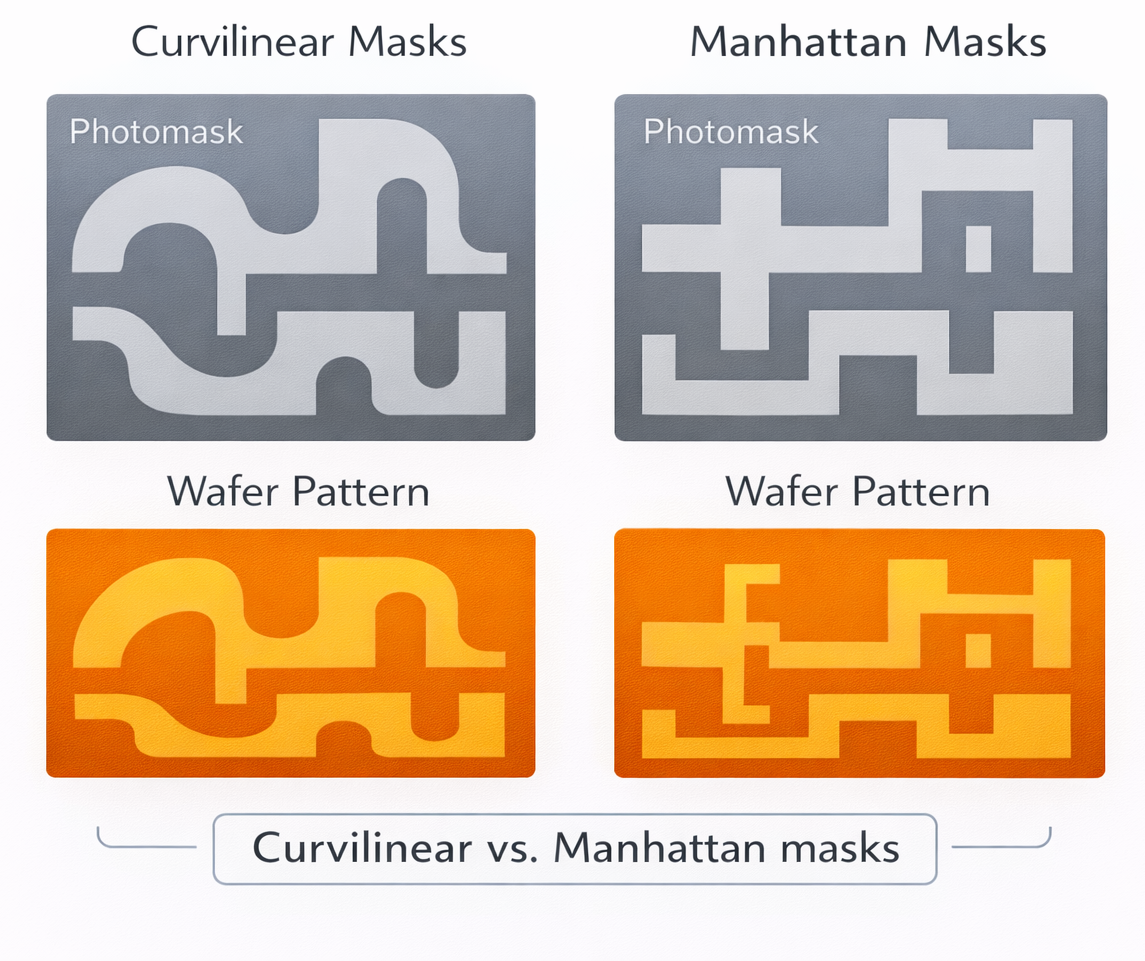
\includegraphics[width=0.7\linewidth]{images/fig3.png}
  \caption{Comparison of traditional Manhattan mask geometries and curvilinear mask representations, along with their corresponding wafer patterns. Curvilinear masks enable improved pattern fidelity and process window by better compensating for diffraction and process effects at advanced technology nodes.}
  \label{fig:curvilinear_vs_manhattan}
\end{figure}

Several studies have shown that GPU acceleration is essential for making curvilinear ILT practical at scale. Shendre et al. provided comprehensive empirical evidence that pixel-based computing on GPU platforms offers inherent advantages for curvilinear photomask optimization, particularly in terms of parallelism and memory efficiency \cite{Shandre2023}. Complementary work by Lan et al. demonstrated how deep learning techniques can further accelerate mask optimization by leveraging GPU-friendly neural models to guide or approximate inverse optimization \cite{Lan2018}. In addition, recent learning-based formulations such as deep neural level-set methods enable near-instant mask optimization, further illustrating the potential of GPU-accelerated learning-assisted ILT workflows \cite{Chen2023DevelSet}.

More recent advances integrate both physics-based optimization and data-driven techniques. Cao et al. explored the application of generative AI in conjunction with ILT to enable efficient synthesis of curvilinear mask patterns, illustrating how modern GPU platforms can support hybrid optimization pipelines \cite{Cao2023}. Yang et al. proposed a GPU-accelerated ILT algorithm that improves contour quality, process window robustness, and curvilinear mask precision, reporting speedups of up to 40$\times$ compared to CPU-based ILT methods \cite{Yang2025}. In addition, Yang et al. discussed the fundamental limitations of conventional OPC and emphasized how ILT and curvilinear masks address critical fidelity challenges in advanced wafer fabrication \cite{Yang2025}. Beyond ILT, GPU acceleration has also been applied to related patterning problems such as multiple-patterning layout decomposition, further underscoring the importance of GPU-based optimization for advanced mask synthesis \cite{Chen2023MatrixCover}.

Together, these innovations demonstrate that curvilinear ILT is both a major driver and a beneficiary of GPU acceleration. The combination of FFT-heavy imaging, gradient-based optimization, and dense mask representations makes GPU-dominant and multi-GPU architectures a necessity rather than an optimization choice.


\subsection{Lithography Toolchain Integration}
While GPU acceleration has transformed lithography simulation and optimization, its full impact is realized only when integrated across the broader lithography toolchain. This includes compatibility with different exposure technologies and downstream mask writing systems that impose additional performance and data management requirements.

\subsubsection{Electron Beam and Deep Ultraviolet Lithography Context}
Electron beam (e-beam) lithography and deep ultraviolet (DUV) lithography continue to play important roles in both mask fabrication and direct-write applications. Lin et al. described use cases for e-beam and DUV lithography across research and manufacturing settings, highlighting their relevance for high-resolution patterning and prototyping \cite{Lin2020}. Tseng et al. reviewed the evolution of electron beam lithography with an emphasis on nanometer-scale device fabrication, discussing advances in tooling, resist processes, and pattern control that enable extremely fine feature sizes \cite{Tseng2003}.

Despite their high resolution, traditional e-beam approaches face throughput limitations that restrict scalability for volume manufacturing. Chang et al. surveyed multiple electron beam techniques aimed at improving throughput for sub-100 nm lithography, noting their potential impact on direct wafer writing and mask patterning \cite{CHANG2001117}. These studies provide important context for understanding why computational lithography, coupled with GPU acceleration, is essential for managing the complexity and data volume associated with modern patterning techniques.

\subsubsection{Integration with Multi-Beam Mask Writers}
Multi-beam mask writers (MBMWs) represent a critical enabling technology for translating curvilinear ILT designs into manufacturable photomasks. By employing thousands of parallel electron beams, MBMWs dramatically reduce mask writing time while maintaining the precision required for advanced nodes, particularly in EUV lithography. However, the adoption of curvilinear masks introduces substantial challenges related to data volume, throughput, and pattern fidelity.

Shamoun et al. discussed the evolving requirements placed on multi-beam mask writers by EUV lithography, emphasizing the need to support higher resolution, improved critical dimension uniformity, red uced line-edge roughness, and zero writer-induced defects \cite{shamoun2021multi}. They also highlighted the growing challenge of managing the large data volumes associated with curvilinear ILT and the importance of close coordination between mask writers and computational lithography tools.

Yasuda et al. reviewed the development of NuFlare Technology’s multi-beam mask writing systems, describing architectural features such as high beam current density, pixel-level dose correction, and charging-effect mitigation designed for high-volume manufacturing of leading-edge masks \cite{yasuda2023recent}. These advances underscore the tight coupling between GPU-accelerated ILT, curvilinear data representations, and downstream mask writing infrastructure.\textcolor{blue}{NuFlare multibeam mask writers also use GPU accelerated Mask Process Correction (MPC) software called PLDC. Here GPU acceleration enables inline MPC for photomasks that adds zero turnaround time for MPC. \cite{Shendre2025} \cite{Nakayamada2024}}

From a system perspective, effective integration between GPU-based lithography computation and multi-beam mask writers is essential for realizing the benefits of curvilinear ILT in production. Managing data growth, preserving pattern fidelity, and sustaining throughput across the toolchain require coordinated advances in algorithms, system architecture, and hardware. As such, MBMW integration represents a key convergence point where GPU-accelerated computation directly influences manufacturing feasibility.


\textcolor{blue}{\subsection{Evaluation Methodology and Benchmarking standards}}
\textcolor{blue}{
To ensure a consistent and transparent analysis of the GPU acceleration claims presented in this survey, the following benchmarking criteria were applied across the reported academic and industrial results. These parameters distinguish between isolated kernel performance and end-to-end workflow efficiency.}

\subsubsection{Baseline Configurations}
Performance speedups (X) are measured against optimized, multi-threaded CPU baselines typical of production-scale Electronic Design Automation (EDA) environments.

\begin{itemize}
  \item \textbf{CPU Baselines}: Standard benchmarks utilize high-performance x86 clusters. For instance, the NVIDIA cuLitho results compare a GPU-accelerated node against a traditional CPU-centric workflow, where 350+ GPUs achieve the throughput equivalent of approximately 40,000 CPU cores (14, 30).
  \item \textbf{Hardware Generations}: Academic results (e.g., OpenILT) primarily utilize data-center grade GPUs (NVIDIA A100/H100) to evaluate scalability (4, 13).
 \end{itemize}

 \subsubsection{Problem Scales and Resolution}

 Computational intensity in this survey is categorized by layout complexity and grid resolution:
 \begin{itemize}
  \item \textbf{Full Chip Scale}: Reflects production-level layouts exceeding several square centimeters, requiring distributed execution across GPU clusters (14, 21).
  \item \textbf{Grid Density}: High-resolution pixel-based ILT (e.g., MultiILT) utilizes dense simulation grids to maintain pattern fidelity, often requiring over 7 GB of VRAM per instance (30).
  \item \textbf{Optimization Depth}: Inverse problems (ILT and SMO) are evaluated over "thousands of iterations" of forward-inverse loops, providing a measure of sustained throughput rather than peak burst performance (2, 10).
 \end{itemize}

 \subsubsection{Precision and Numerical Fidelity}

 Numerical precision is a critical factor in balancing throughput and lithographic quality:
 \begin{itemize}
  \item \textbf{Standard Precision}: Unless otherwise noted, FFT-based imaging and PDE solvers utilize single-precision (FP32), which is the industry standard for maintaining edge placement error (EPE) accuracy while maximizing GPU arithmetic intensity (4, 20).
  \item \textbf{AI assisted precision}: Hybrid workflows incorporating neural surrogates often leverage mixed-precision (FP16/BF16) for inference stages to achieve the reported 2
  performance boost without sacrificing final mask manufacturability (29, 30).
 \end{itemize}

 \subsubsection{Workflow Scope: Isolated vs. End to End}

 We distinguish between two primary execution models to clarify the source of speedup:
 \begin{itemize}
  \item \textbf{Isolated Kernels}: Early and transitional commercial tools (e.g., S-Litho) often reflect "kernel-only" acceleration of FFT-based imaging or specific resist calculations, where performance is frequently limited by host-device data transfer overhead (11, 40).
  \item \textbf{End to End (GPU-Resident)}: Modern GPU-first platforms (e.g., cuLitho, OpenILT) report "end-to-end" metrics. In these models, the entire optimization loop—including optical simulation, resist modeling, and gradient evaluation—remains device-resident to eliminate communication bottlenecks (4, 14, 23).
 \end{itemize}

  
\subsection{Performance Benchmarks and System-Level Impact}


Quantifying the performance impact of GPU acceleration in computational lithography is challenging due to differences in workload characteristics, process assumptions, hardware configurations, and optimization objectives across studies. Rather than presenting a unified benchmarking methodology, this section summarizes representative performance results reported in academic and industrial literature, with the goal of illustrating broad system-level trends rather than absolute performance rankings.

Early analytical work emphasized the importance of balancing simulation accuracy and computational cost, providing closed-form methods to estimate error bounds and convergence behavior for lithography simulation techniques \cite{smith2003methods}. These analyses remain relevant in the GPU era, as acceleration enables more accurate models to be evaluated within practical time constraints rather than simply speeding up existing approximations.

Across a wide range of reported studies, GPU acceleration consistently delivers order-of-magnitude speedups for computationally dominant lithography kernels. Table \ref{tab:gpu_speedups} summarizes representative speedup results for GPU-accelerated OPC and ILT workflows, including academic prototypes, early commercial tools, and recent industrial platforms. Academic GPU-accelerated ILT implementations typically report speedups of 15× or greater relative to optimized CPU baselines, particularly for FFT-heavy imaging and gradient-based optimization in curvilinear mask synthesis. Early commercial GPU-enabled ILT tools demonstrated 10–20× speedups, largely by accelerating optical simulation and edge operations while retaining CPU-driven workflow control.

Industrial platforms provide the clearest evidence of system-level impact. NVIDIA’s cuLitho platform reports 40–60× speedups compared to traditional CPU-based lithography flows, achieved through full-pipeline GPU residency, large-scale parallel execution, and optimized data movement across multi-GPU systems. These gains are further amplified by the integration of AI-assisted workflows, which have been reported to deliver an additional ~2× performance improvement for selected optimization tasks, as reflected in the industrial benchmarks summarized in Table \ref{tab:gpu_speedups}.

Memory footprint is an equally important consideration for scalable GPU execution. Different ILT algorithms exhibit substantially different GPU memory requirements depending on mask representation, resolution, and optimization strategy. Table \ref{tab:ilt_gpu_memory} compares representative GPU memory footprints and corresponding optimization strategies reported for several ILT implementations. Pixel-based and high-resolution curvilinear ILT approaches can require multiple gigabytes of device memory per instance, while memory-aware tiling and morphological representations significantly reduce per-device requirements. Large-scale industrial platforms address these challenges through distributed execution across hundreds of GPUs, effectively trading aggregate device memory for throughput and scalability.

Collectively, the benchmark results summarized in Tables \ref{tab:gpu_speedups} and \ref{tab:ilt_gpu_memory} demonstrate that GPU acceleration fundamentally reshapes the performance envelope of computational lithography. By enabling faster simulation, higher-fidelity models, and more robust optimization, GPU-based systems expand the practical design space rather than merely reducing execution time.

  
\begin{table}[t]
\centering
\small
\setlength{\tabcolsep}{6pt}
\begin{tabularx}{\linewidth}{|l|c|X|}
\hline
\textbf{Library / Algorithm} & \textbf{Speedup vs. CPU} & \textbf{Key Notes} \\
\hline
NVIDIA cuLitho & 40--60$\times$ &
350+ GPUs replace $\sim$40{,}000 CPUs for TSMC; additional $\sim$2$\times$ boost from AI workflow integration; enables overnight mask generation \\ 
\hline
Modern custom GPU ILT (Academic) & $\ge$15$\times$ &
Improved convergence and memory efficiency, especially for curvilinear shapes \\ 
\hline
Early commercial GPU ILT & 10--20$\times$ &
Acceleration of simulation and edge operations; early benchmarks (circa 2020) showed $>$10$\times$ gains \\ 
\hline
GAN/AI-enhanced GPU OPC/ILT & $\sim$50\% reduction &
Deep learning integration halves computation time for curvilinear mask optimization \\ 
\hline
\end{tabularx}
\caption{Reported GPU-accelerated ILT and OPC algorithm performance compared to CPU baselines.}
\label{tab:gpu_speedups}
\end{table}

\begin{table}[t]
\centering
\small
\setlength{\tabcolsep}{6pt}
\begin{tabularx}{\linewidth}{|l|c|X|}
\hline
\textbf{Algorithm} & \textbf{Peak GPU Memory} & \textbf{Key Optimization} \\ 
\hline
MultiILT & 7.2 GB &
High-resolution pixel phase; detailed curvilinear representation \\ 
\hline
curvyILT & 0.6 GB &
Morphological operations with reduced post-processing intensity \\ 
\hline
cuLitho & N/A (large total VRAM) &
Distributed execution across 350--500 GPUs with bottleneck minimization \\ 
\hline
TrueMask ILT & N/A (optimized) &
Full-chip curvilinear mask rasterization with memory-aware tiling \\ 
\hline
\end{tabularx}
\caption{Comparison of ILT algorithm GPU memory requirements and optimization strategies.}
\label{tab:ilt_gpu_memory}
\end{table}



\subsection{Industry Adoption and Manufacturing Impact}
The performance improvements enabled by GPU acceleration have driven rapid adoption of GPU-based computational lithography frameworks across the semiconductor industry. Major stakeholders—including equipment vendors, foundries, and EDA providers—have increasingly embraced GPU-centric architectures to address the growing complexity of advanced process nodes.

A prominent example is the deployment of NVIDIA’s cuLitho platform in partnership with leading foundries such as TSMC. Reported deployments demonstrate that hundreds of modern GPUs can replace tens of thousands of CPU cores, delivering equivalent or superior throughput while dramatically reducing power consumption and physical footprint. These gains have immediate operational benefits, including lower energy costs, reduced data center space requirements, and improved sustainability metrics.

Beyond raw performance, GPU acceleration enables qualitatively new manufacturing capabilities. While inverse lithography and curvilinear mask techniques have been studied in the literature for more than two decades, their full-chip deployment was historically impractical due to excessive computation time. GPU-accelerated platforms now make large-scale ILT and curvilinear optimization feasible within production timelines, allowing foundries to adopt more aggressive resolution enhancement strategies at advanced nodes.

The integration of generative AI and machine learning further amplifies these benefits. By combining GPU-accelerated physics-based simulation with AI-driven optimization, modern lithography workflows can explore larger design spaces, identify non-intuitive solutions, and converge more rapidly. Reported results indicate that AI-assisted pipelines can reduce computation time by approximately 50\% on top of existing GPU acceleration, reinforcing the role of GPUs as both numerical and learning accelerators.

From a manufacturing perspective, these advances shorten development cycles for new technology nodes, accelerate mask qualification, and improve yield through more robust patterning solutions. They also enable tighter coupling between computational lithography, mask writing, and wafer fabrication, supporting rapid iteration and faster time-to-market. As a result, GPU-accelerated lithography has transitioned from an optimization option to a strategic enabler for next-generation semiconductor manufacturing.

\subsection{Architectural Lessons Learned} 
The systems surveyed in this section—spanning academic frameworks, industrial platforms, and production deployments—collectively reveal several architectural lessons that are critical for scalable GPU acceleration in computational lithography.

\begin{itemize}
	\item \textbf{End-to-End GPU Residency Is Essential for Scalability}: Across both academic and industrial systems, designs that maintain optical simulation, resist modeling, and inverse optimization entirely on the GPU consistently outperform hybrid CPU–GPU pipelines. While early approaches achieved meaningful kernel-level speedups, frequent host–device data transfers and CPU-driven control flow limited scalability. Platforms such as cuLitho and GPU-centric ILT frameworks demonstrate that full-pipeline GPU residency is a prerequisite for sustaining high throughput across thousands of tightly coupled optimization iterations.
	
	\item \textbf{Memory Footprint, Not Compute Throughput, Is the Primary Bottleneck}: Although lithography workloads are computationally intensive, memory capacity and data movement increasingly dominate system design decisions. High-resolution curvilinear ILT and stochastic resist modeling can require several gigabytes of device memory per instance, constraining single-GPU execution. Successful systems therefore employ memory-aware tiling, hierarchical representations, and multi-GPU partitioning to balance fidelity with scalability.

\item \textbf{Multi-GPU and Cluster Architectures Are Mandatory at Production Scale}: Single-GPU and even single-node multi-GPU systems are insufficient for full-chip inverse lithography and robust optimization at advanced nodes. Production deployments leverage GPU clusters to parallelize across spatial domains, illumination conditions, and optimization ensembles. This embarrassingly parallel structure enables near-linear scaling when communication is minimized and data locality is preserved.

\item \textbf{Curvilinear ILT Drives Architectural Co-Design}: The adoption of curvilinear mask representations fundamentally changes computational requirements. Dense, continuous optimization variables increase both arithmetic intensity and memory pressure, requiring co-design across algorithms, data structures, and hardware. Systems that treat curvilinear ILT as a drop-in replacement for OPC often fail to scale, whereas GPU-first architectures explicitly designed for pixel-level parallelism achieve superior performance and manufacturability outcomes.

\item \textbf{Hybrid AI–Physics Pipelines Require Tight Integration}: Learning-assisted ILT and generative AI workflows amplify GPU utilization but only when tightly integrated with physics-based solvers. Loosely coupled AI accelerators introduce additional data movement and synchronization overhead, eroding gains. Successful designs unify neural inference, gradient computation, and lithography simulation within a single GPU-resident execution model.

\item \textbf{Toolchain Integration Determines Real-World Impact}: Finally, computational gains translate into manufacturing value only when integrated across the lithography toolchain. Compatibility with multi-beam mask writers, support for large curvilinear data volumes, and alignment with foundry workflows are essential. Systems that consider GPU acceleration in isolation risk optimizing algorithms that cannot be deployed at scale.
\end{itemize}

In summary, scalable computational lithography requires holistic, GPU-centric system design. The architectural lessons distilled in this section underscore that performance gains arise not from isolated optimizations, but from coordinated advances across algorithms, memory management, parallel execution, and toolchain integration.



\section{Open Challenges and Research Roadmap}
Despite significant advances in GPU-accelerated computational lithography, several open challenges remain that will shape future research and system design. As lithography continues to push toward smaller feature sizes, higher numerical apertures, and tighter process windows, computational demands are increasing faster than hardware performance alone can address. This section outlines key limitations and presents a roadmap for future research at the intersection of lithography, high-performance computing, and artificial intelligence.

\subsection{Physical and Modeling Challenges in Next-Generation Lithography}
Extreme ultraviolet (EUV) lithography has become indispensable for advanced technology nodes, yet it introduces new challenges that directly impact computational lithography. As noted by Levinson, exposure tool reliability—particularly EUV light source stability—and mask contamination remain critical bottlenecks affecting productivity and yield \cite{levinson2018current}. At the same time, resist performance poses fundamental challenges. Photon shot noise at EUV wavelengths leads to stochastic variability that cannot be mitigated without higher exposure doses, which in turn exacerbate throughput and power constraints.

These physical limitations significantly increase the complexity of computational lithography models. Future EUV systems will require more accurate resist and stochastic modeling, potentially involving non–chemically amplified resists and higher-fidelity reaction–diffusion or Monte Carlo simulations. As a result, next-generation computational lithography is expected to be substantially more expensive, reinforcing the need for scalable GPU-accelerated and cluster-based solutions.

\subsection{Performance, Accuracy, and AI Integration Tradeoffs}
Achieving both high accuracy and fast turnaround time remains a central challenge. While GPU acceleration enables order-of-magnitude speedups, increasing model fidelity—particularly for EUV resist and variability analysis—quickly consumes available computational resources. Negele et al. emphasize the need for faster simulations, improved accuracy, and tighter integration of AI techniques to sustain progress in lithography \cite{negele2025}. At the system level, this raises important questions about how simulation fidelity, optimization convergence, and hardware utilization should be balanced.

The rapid pace of GPU innovation presents both opportunities and challenges. New GPU architectures could be brought into production faster than traditional lithography tools, potentially accelerating Moore’s law itself. However, realizing this potential requires deeper understanding of the compute–design–manufacturing feedback loop, including how AI-accelerated lithography influences process development, node ramp-up, and yield learning. This feedback loop remains underexplored and represents an important research direction.

\subsection{Integration of Generative AI for Mask Synthesis}
Generative artificial intelligence has emerged as a powerful complement to physics-based computational lithography, particularly for accelerating mask synthesis and inverse optimization workflows. Traditional lithography modeling relies on rigorous optical and resist simulations that are computationally expensive, even on modern GPU platforms. While neural networks can approximate these models, accuracy degradation and limited training data have historically impeded industrial adoption.

Recent work has begun to address these limitations through data-centric and hybrid approaches. Liu et al. proposed a lithography-aware data augmentation (LADA) framework that combines pretrained neural lithography models with adversarial sampling using generative models to synthesize informative, in-distribution mask patterns, improving robustness and narrowing the performance gap between training and testing data \cite{liu2023adversarial}. Related efforts have explored convolutional neural network–based data augmentation strategies specifically tailored to EUV lithography simulation, further highlighting the importance of dataset quality for AI-driven models \cite{Tanabe2022}.

Generative models have also been applied directly to mask and layout synthesis. Zhang et al. introduced a framework that synthesizes critical mask and layout patterns using a combination of multilayer perceptrons, conditional generative adversarial networks, and U-Net architectures, demonstrating significant reductions in edge placement error variance and improved lithography model accuracy when trained on synthesized critical patterns \cite{zhang2025synthesis}. Chen et al. proposed a deep neural level-set formulation for instant mask optimization, illustrating how learning-based approaches can dramatically reduce turnaround time when deployed on GPU platforms \cite{Chen2023DevelSet}. Related inverse phase optimization problems in computational optics have also benefited from end-to-end learning, reinforcing the broader applicability of learning-based inverse design techniques to lithography \cite{Shi2022Hologram}.

\subsection{Expansion of Open-Source GPU Lithography Frameworks}
Open-source platforms play a crucial role in accelerating innovation and reproducibility in computational lithography. However, progress in AI-driven lithography is often constrained by the lack of large, high-quality datasets and standardized evaluation pipelines. To address this gap, Zheng et al. introduced LithoBench, a large-scale dataset and benchmarking framework designed for deep learning–based lithography simulation and mask optimization \cite{zheng2023lithobench}. LithoBench enables systematic comparison of neural models and supports rapid experimentation with AI-driven approaches.

In parallel, Chen et al. presented an open-source differentiable lithography framework based on GPU-accelerated differentiable programming \cite{chen2024open}. By modeling optical imaging and resolution enhancement techniques as differentiable components, the framework enables gradient-based optimization using modern machine learning toolchains. The availability of open frameworks such as TorchLitho lowers the barrier to entry for researchers and promotes collaboration, but also raises challenges related to validation, scalability, and alignment with industrial requirements.

\subsection{AI-Driven Computational Lithography}
Beyond generative mask synthesis, AI-driven computational lithography encompasses a broader class of learning-based methods applied to source–mask optimization, inverse lithography, resist modeling, and process variation analysis. By constructing surrogate models, differentiable simulators, and physics-informed neural networks, these approaches aim to reduce reliance on repeated, expensive forward simulations while enabling uncertainty-aware optimization.

Shi et al. demonstrated that carefully designed, physics-based feature vectors can significantly improve the generality and robustness of machine learning models for computational lithography, enabling a universal learning-based framework when combined with deep neural architectures \cite{shi2020ai}. Complementary work by Liu et al. explored the use of machine learning software and hardware platforms for mask synthesis, emphasizing the importance of GPU acceleration and algorithm–hardware co-design for practical deployment \cite{liu2020mask}. Efficient GPU inference engines further support deployment of learning-based lithography models, particularly when tight latency and throughput constraints must be met \cite{PhoneBit2019}.

From a systems perspective, AI-driven lithography benefits directly from advances in GPU architectures and large-scale training frameworks. Large-scale GPU training frameworks demonstrate the feasibility of training lithography-scale models, reinforcing the role of GPUs as the unifying platform for both physics-based and learning-based computation \cite{HugeCTR2022}. As lithography workflows increasingly span multiple tools and computing resources, distributed and split-learning paradigms may become relevant for collaborative or resource-constrained settings, although their application to production lithography remains an open research question \cite{Lin2024SplitLearning}.

Despite their promise, significant challenges remain. Dataset generation remains costly, interpretability of learned models is limited, and compliance with foundry design rules and verification flows is not guaranteed. Addressing these issues—while ensuring tight integration between AI models and GPU-resident physics solvers—constitutes a central component of the research roadmap for next-generation computational lithography.


\section{Roadmap and Outlook}

\subsection{Vendor Dependence and CUDA dominance}
While the paper correctly identifies CUDA as the industry standard due to its mature compiler support and highly optimized libraries (like those used in NVIDIA cuLitho), it highlights a significant risk of vendor lock-in.
\begin{itemize}
  \item The Trade-off: The high performance reported (up to 40-60x) is often tied to hardware-specific features that make migrating to other GPU vendors difficult without substantial code rewrites.
  \item Implication: Foundries and EDA providers become dependent on a single hardware roadmap, which can impact long-term procurement strategies and cost controls.

\end{itemize}

\subsection{Alternative GPU Ecosystems and Portability}
The discussion on OpenCL can be strengthened by framing it not just as a "weaker" alternative, but as a necessary standard for cross-platform portability.
\begin{itemize}
  \item  OpenCL vs. CUDA: While OpenCL allows code to run across NVIDIA, AMD, and Intel GPUs, it currently lacks the vendor-optimized, lithography-specific libraries (such as FFT and linear algebra) that drive the performance of platforms like cuLitho.
  \item Emerging Standards: You could mention the potential role of SYCL or HIP as middle-ground solutions that aim to offer performance similar to CUDA while maintaining a path to multi-vendor hardware support.
\end{itemize}

\subsection{Implications for System Architecture}
The move toward full-pipeline GPU residency (where everything from optical simulation to inverse optimization stays on the device) further complicates portability.
\begin{itemize}
  \item Hardware Sensitivity: Because these end-to-end models are designed to minimize host-device data movement, they are often finely tuned to the specific memory hierarchy and interconnect speeds (e.g., NVLink) of a particular vendor's architecture.
  \item The "Portability Tax": Achieving true neutrality often requires adopting higher-level abstractions that may introduce the very data movement bottlenecks the paper argues against.
  
\end{itemize}

Looking forward, the evolution of computational lithography will be shaped by the convergence of three forces: increasing physical complexity at advanced nodes, rapid advances in GPU and accelerator architectures, and growing integration of AI into simulation and optimization workflows. Addressing open challenges will require holistic system-level design that unifies physics-based modeling, learning-based surrogates, memory-efficient execution, and scalable cluster architectures. Key directions on the research roadmap include:
\begin{itemize}
	\item GPU-first and cluster-native lithography pipelines capable of sustaining full-chip ILT and stochastic EUV modeling.

 \item Hybrid AI–physics frameworks that combine generative models with rigorous simulation while preserving accuracy and manufacturability.

\item Expanded open-source ecosystems with standardized datasets, benchmarks, and differentiable lithography components.

\item Deeper integration with manufacturing toolchains, including multi-beam mask writers and foundry verification flows.

\end{itemize}
Together, these efforts will determine whether computational lithography can continue to scale alongside semiconductor manufacturing, enabling both near-term productivity gains and long-term innovation beyond traditional scaling limits.
  
  
\section{Conclusion}
Computational lithography has evolved from a specialized simulation task into a central pillar of advanced semiconductor manufacturing, driven by the increasing complexity of optical systems, resist behavior, and process variability at modern technology nodes. As this survey has shown, GPUs are no longer optional accelerators in this domain; they have become foundational computing substrates that enable the scale, fidelity, and turnaround times required for contemporary lithography workflows. From FFT-based optical imaging and stochastic resist modeling to large-scale inverse optimization and curvilinear mask synthesis, GPU architectures align naturally with the massive parallelism inherent in lithographic computation.

Equally important, computational lithography has become a convergent field at the intersection of high-performance computing and artificial intelligence. GPU-accelerated physics-based solvers now coexist with learning-based surrogates, differentiable pipelines, and generative models that together expand the feasible design space and enable rapid exploration of complex optimization landscapes. Industrial platforms and open research frameworks alike demonstrate that performance gains arise not from isolated kernel acceleration, but from holistic, GPU-centric system design that tightly integrates algorithms, memory management, and parallel execution across multi-GPU and cluster-scale environments.

By consolidating algorithmic foundations, architectural insights, performance benchmarks, and industrial adoption trends, this survey provides a unified taxonomy and roadmap for GPU acceleration in computational lithography. The resulting perspective positions the field to address the challenges of next-generation EUV systems, curvilinear mask proliferation, and AI-assisted optimization. As semiconductor manufacturing enters an era defined by both physical limits and unprecedented computational opportunity, GPU-enabled computational lithography stands as a key enabler for innovation over the next decade and beyond.
  

%\bibliographystyle{sn-mathphys-num}  % or sn basic / sn chicago etc., matching your class
\bibliography{sn-bibliography}% common bib file
%% if required, the content of .bbl file can be included here once bbl is generated
%%\input sn article.bbl

\end{document}
